\documentclass{scrartcl}
\usepackage[utf8]{inputenc}
\usepackage[english]{babel} % Trennung nach der neuen deutschen Rechtschreibung
\usepackage[utf8]{inputenc}
\usepackage[T1]{fontenc}
\usepackage{lmodern}
\usepackage{subcaption}
\usepackage{chemformula}
\usepackage{placeins}
\usepackage{multirow}
\usepackage{enumitem}
\usepackage{amssymb}
\usepackage{amsmath} % Erweiterte Mathematik-Umgebung
\usepackage{amsfonts} % zusätzliche Mathematik-Schrifttypen (v.a. \mathbb für Mengen)
\usepackage{ulem}
\usepackage{amsthm}
\usepackage{graphics}%soll beim Graphiken einfügen hilfreich sein
\usepackage{graphicx}
\usepackage{wrapfig}%lässt Textumflossene Bildeinbindung zu
\usepackage{epstopdf}%soll eps in pdf umwandeln
\usepackage{placeins}
\usepackage{amsthm}
\usepackage{subcaption}
\usepackage{wrapfig}
\usepackage{hyperref}
\usepackage{ragged2e}

\usepackage[a4paper, portrait, margin=2.5cm]{geometry}

\begin{document}
\begin{titlepage}
    \begin{center}
        \vspace*{1cm}
        \Huge
        \textbf{X-rays}
        
        \vspace{0.5cm}
        \LARGE
        Advanced Lab Course
        
        \vspace{1.5cm}
        \textbf{Louis-Hendrik Barboutie (020157041C) and Florence Schmerber (0201845640)}
        
        \vspace{1cm}
        Under the supervision of Himanshu Phirke
        \vfill
        

        
\includegraphics[width=0.4\textwidth]{logo_uni.jpg}
        
        \Large
        17th March 2022
    \end{center}
\end{titlepage}

\clearpage

\tableofcontents

\listoffigures
	
\clearpage

\section{Introduction}
X-rays are high-energy electromagnetic radiation, which are commonly used the the medical world for imaging purposes. During this experiment we will focus our interest on the X-rays produced by a Molybdenum anode. In a first step, we will study the characteristics of the anode, then investigate the Duane-Hunt law and Mosley's law, to determine Planck's constant and Rydberg's constant experimentally. In a second step, we will study the effect of X-rays on air, how we can characterize the ionization of the air hit by X-rays. In a final step we will be making a Laue diagram of a Lithium Fluoride crystal and study its laticces structure.\\ \begin{wrapfigure}[15]{r}{0.4\textwidth}
    \centering
    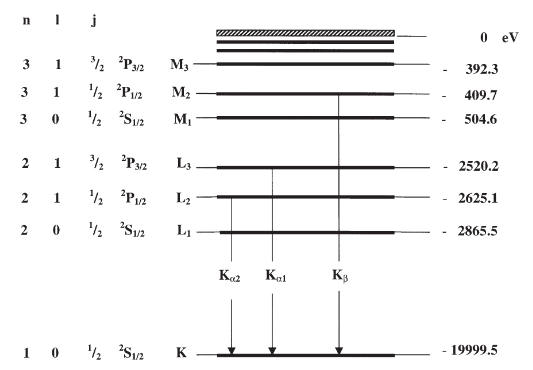
\includegraphics[width=7cm]{MolybdenumEnergyTransitions.png}
    \caption{Molybdenum energy transitions}
    \label{fig:molybdenumEnergyTransitions}
\end{wrapfigure} The Molybdenum anode emits X-rays when it gets hit by electrons with high enough kinetic energy. When an electron collides inelastically with a Molybdenum atom, an electrons inside the Molybdenum atom jumps one or two energy levels higher, into an excited state. When the electron returns back to the ground state, it emits electromagnetic radiation. In the case of the Molybdenum, it is X-rays. Most energy transitions do are not very big, but the most remarkable, and therefore called characteristic transitions for Molybdenum are from the state $n=3$ and $n=2$ to the ground state $n=1$ and are called $K_{\beta}$ and $K_{\alpha}$ transitions respectively (see figure~(\ref{fig:molybdenumEnergyTransitions})). When the intensity of the emitted X-rays is recorded, called the Bremsstrahlungs-spectrum, one obtains high peaks in intensity for the characteristic transitions. These transitions are also unique for every element, and allow for the identification of unknown elements. \\ Since X-rays have high energy, they have the potential to ionize air, ie. to rip off electrons from the molecules. The air then gets charged, and can conduct electric current. \\ X-rays can be scattered like light using a crystal, which is in simple terms a periodic arrangement of atoms. It is similar to a double slit diffraction, except that each atom in the crystal acts as a slit. The pattern observed is therefore different, but characteristic to the crystal. It can show what type of crystalline structure it has. Lithium Fluoride crystals for example have a face-center-cubic structure.

\section{Experiment}

\subsection{Setup}

\noindent The setup used for the experiment is represented in figure~(\ref{fig:test2}). It has several parameter inputs on the left, an X-ray emitting tube in the center and an experiment area with a detector, crystal spectrometer and goniometer on the right. It allows us to do $\theta-2\theta$ scans of the X-ray intensity emitted by the X-ray tube. The schematic of the X-ray tube can be found in figure~(\ref{fig:test1}). A high voltage is applied on the cathode, which will heat up and release electrons. These electrons then go to the anode where they release part of their kinetic energy, which gets converted into X-rays. The X-rays then scatter on the crystal and the detector measures the intensity the scattered rays. The goniometer allows to simultaniously rotate the crystal and the detector, so that the angle between the incident ray is always $2\theta$, while the angle between the crystal and the ray and between the crystal and the detector is $\theta$. \\ The experimental area can be swapped for a capacitor for the study of the ionization of air, and then swapped with a holding cell for a crystal and photosensitive film.
\begin{figure}
    \centering
    \begin{subfigure}{0.4\textwidth}
    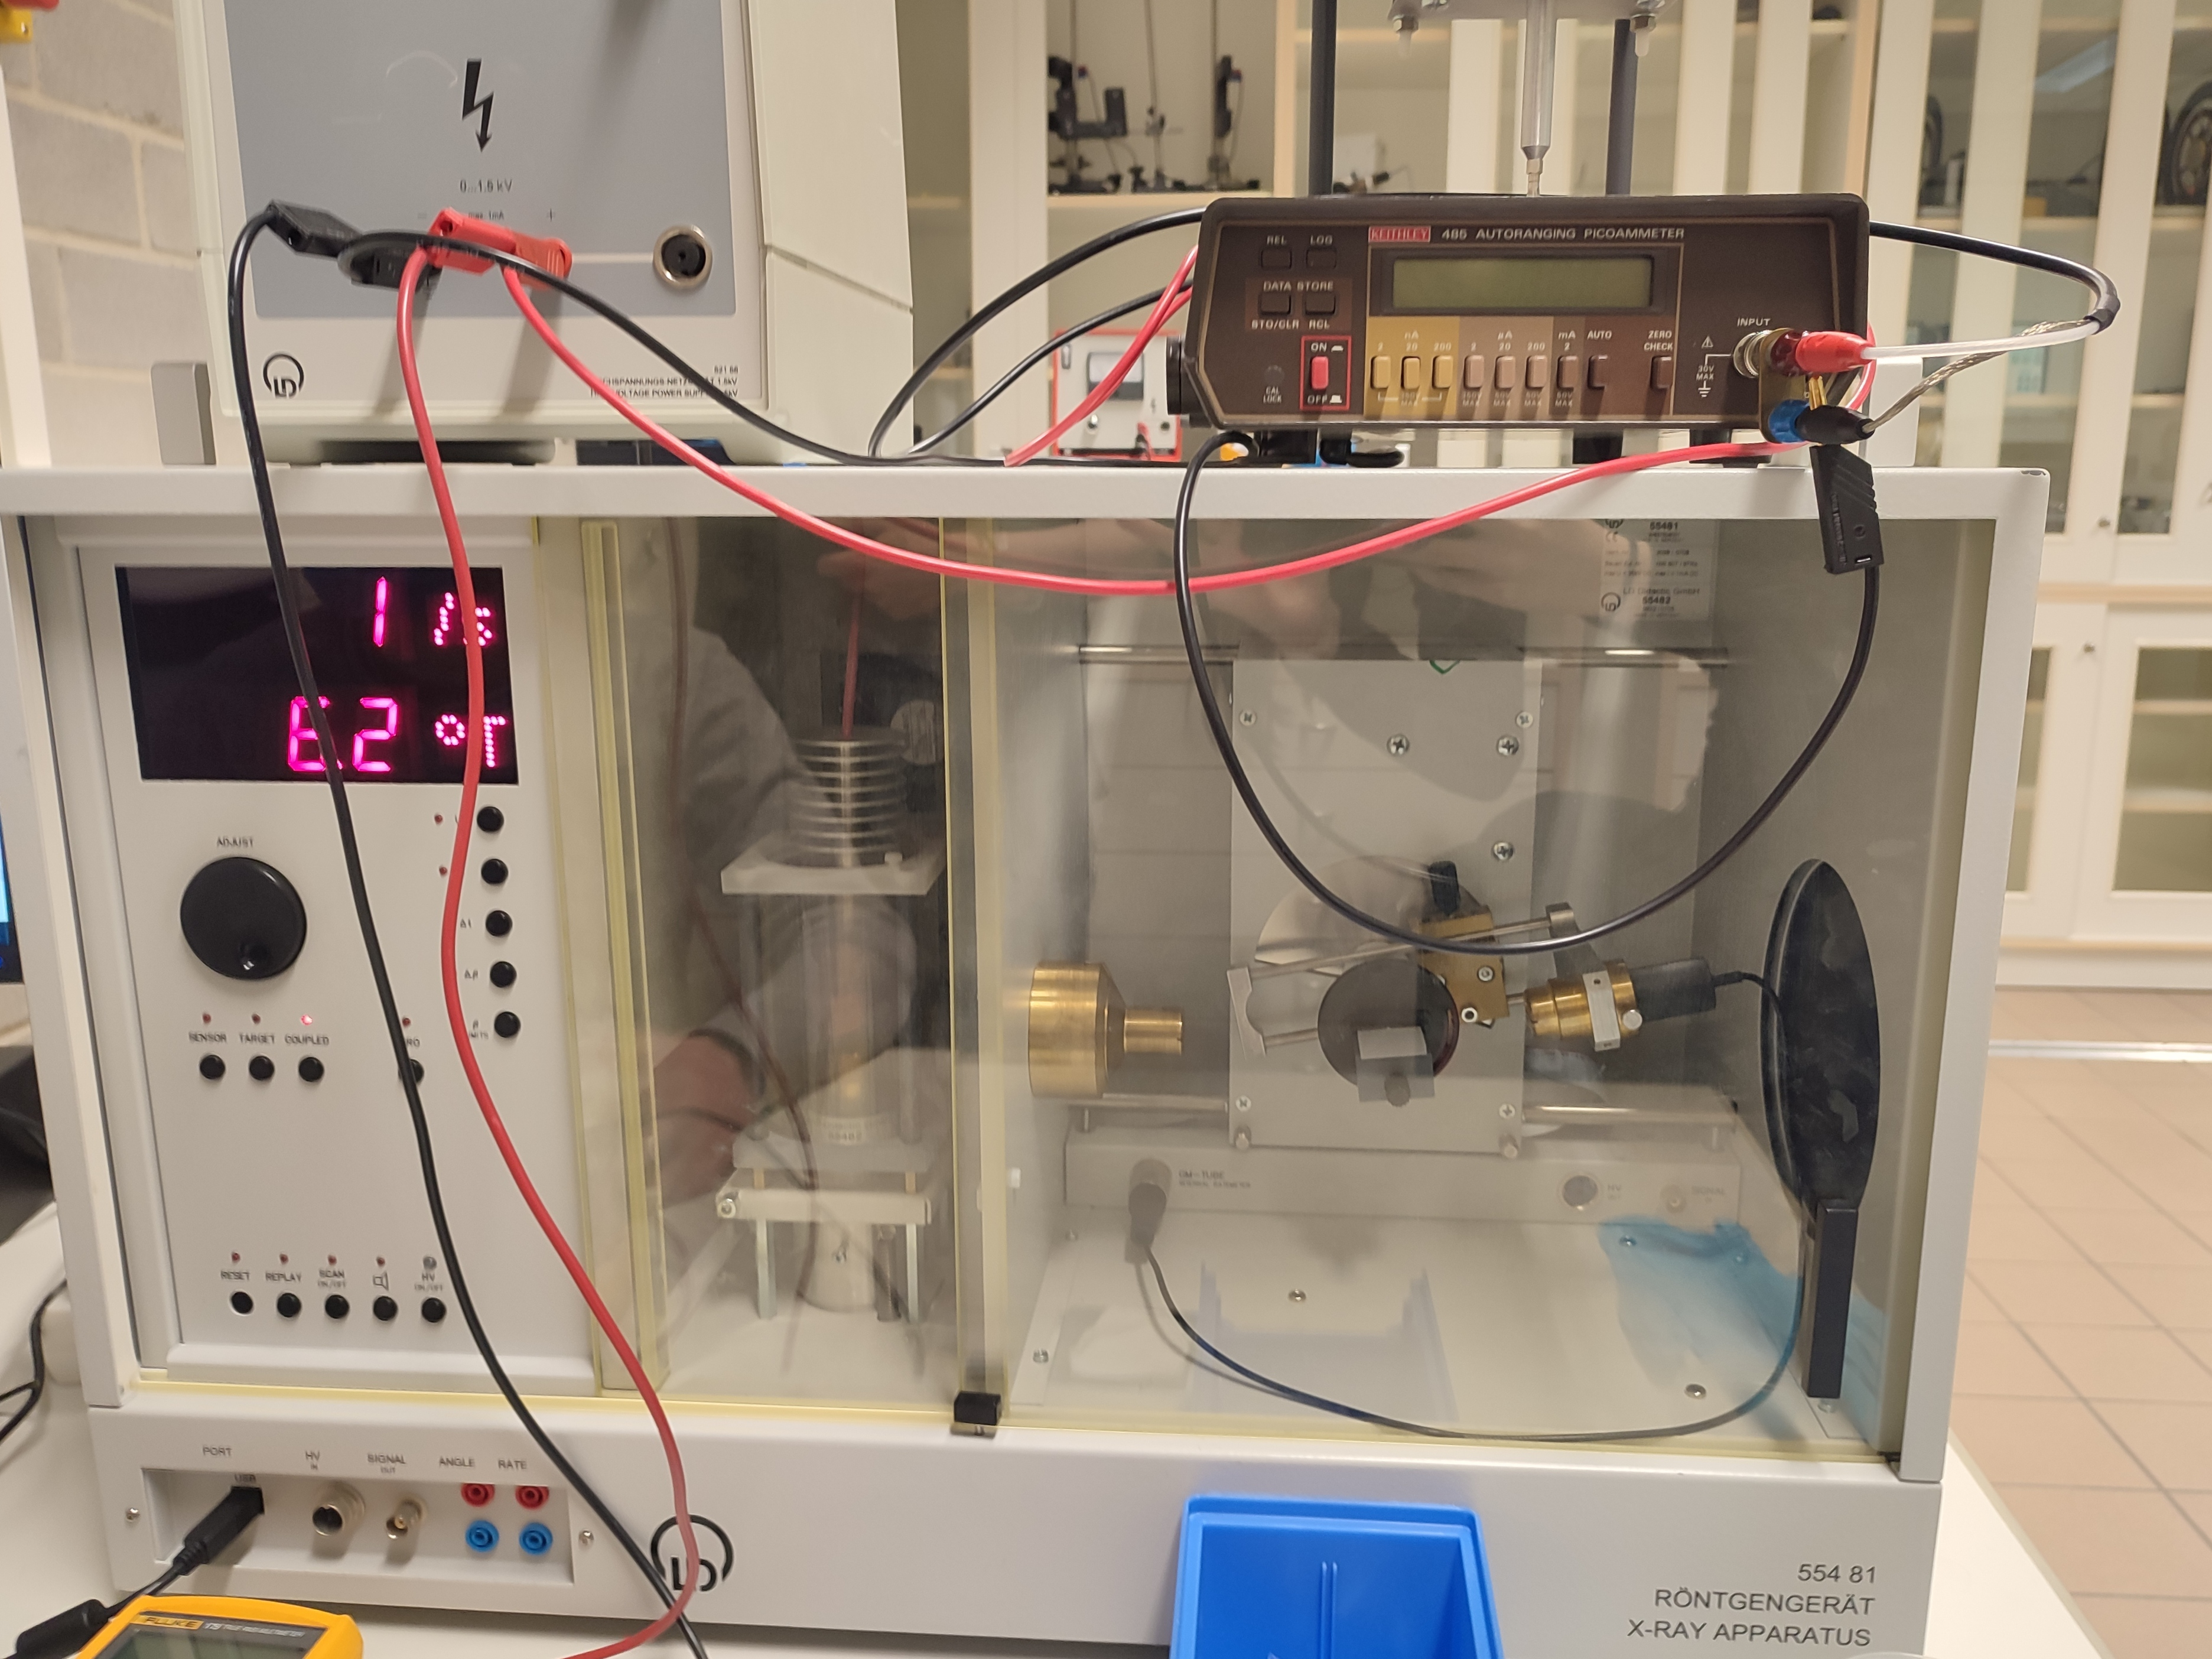
\includegraphics[width=\textwidth]{1647529200496.jpg}
    \captionof{figure}{Experimental device}
    \label{fig:test2}
    \end{subfigure}
    \hfill
    \begin{subfigure}{0.4\textwidth}
    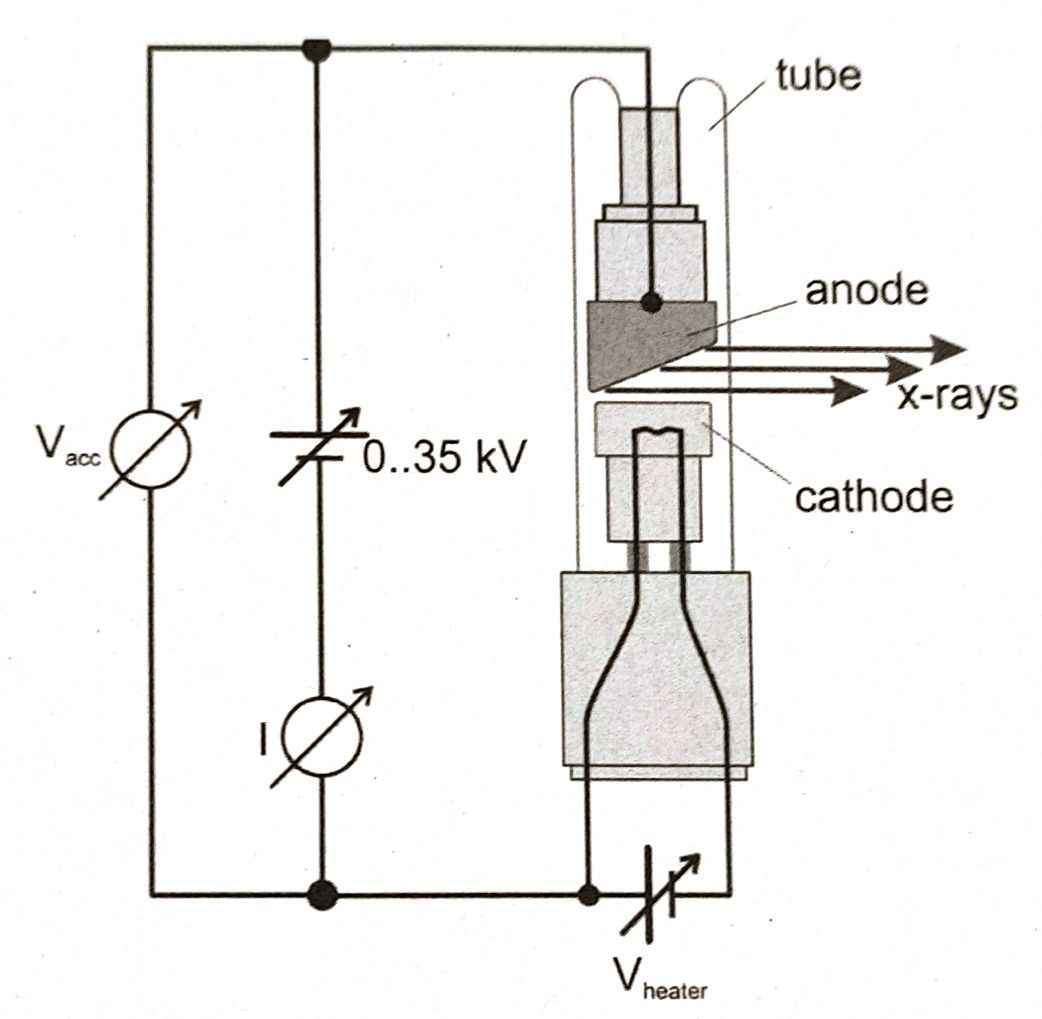
\includegraphics[width=\textwidth]{x_ray_2.jpg}
    \captionof{figure}{X-ray tube}
    \label{fig:test1}
    \end{subfigure}
    \caption{Experimental Setup and schematic of an X-ray tube}
\end{figure}

\section{Results and discussion}

\subsection{Spectrum of X-rays produced by a Mo anode}

We perform a $\theta-2\theta$ scan with a sodium crystal as spectrometer, with the parameters in table(\ref{tab:parameterBremsstrahlungsSpectrum}).

\begin{table}[!ht]
    \centering
    \begin{tabular}{c|c|c|c|c|c}
    Voltage (kV) & Current (mA) & $\Delta \beta$ & $\beta_{min}$   &  $\beta_{max}$   &  Acquisition time  \\ \hline
    35  & 1 & 0,1° & 2° & 25° & 10 \\
    \end{tabular}
    \caption{Parameters to produce the Bremstrahlung spectrum}
    \label{tab:parameterBremsstrahlungsSpectrum}
\end{table}

\noindent The resulting spectrum is presented in figure~(\ref{fig:bremsstrahlungSpectrum}):

\begin{figure}[!ht]
    \centering
    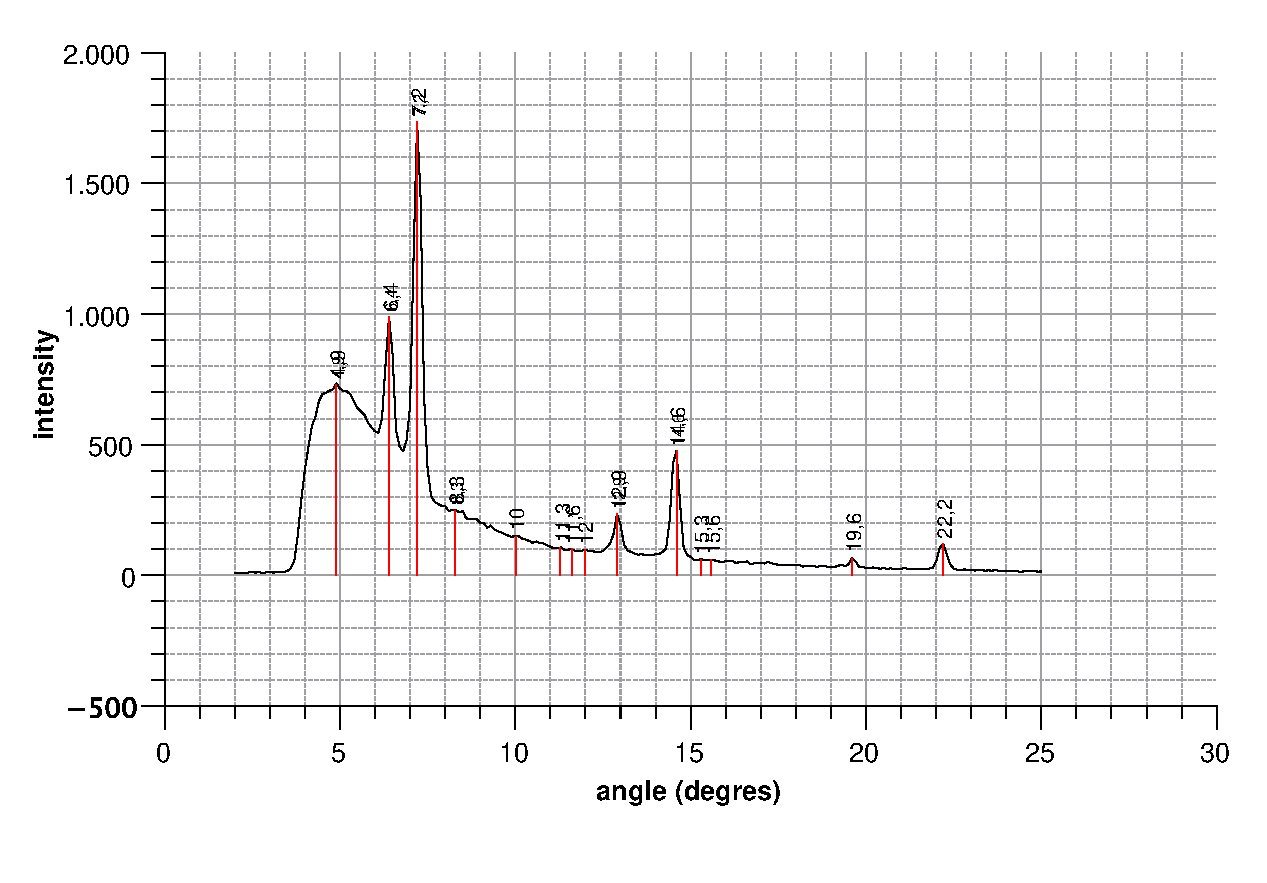
\includegraphics[width=0.8\textwidth]{firstmeasurement.eps}
    \caption{The Bremstrahlung spectrum of Molybdenum}
    \label{fig:bremsstrahlungSpectrum}
\end{figure}

\noindent We can observe the characteristic peaks which correspond to the emission lines $K_{\alpha}$ and $K_{\beta}$. We can use Bragg's law (equation~(\ref{braggLaw})) \cite{braggLaw} to find the wavelengths corresponding to the peaks. \begin{equation}n\lambda = 2dsin(\beta) \label{braggLaw}\end{equation} where d = 272.01 pm is the distance between the lattices of the sodium crystal and $\beta$ the diffraction angle. The calculation of the theoretical values expected for $K_\alpha$ and $K_\beta$, which are calculated in the appendix. The first peak of each pair of peaks corresponds to the $K_\beta$, since it has smaller wavelength and therefore higher energy. On the other hand, the $K_\alpha$ peaks have bigger wavelengths and therefore smaller energies. Several orders of the peaks appear, and we can use all of them to take an average.
The corresponding wavelengths for $K_\beta$ can be found in table~(\ref{tab:kBetaWavelength}), and for $K_\alpha$ in table~(\ref{tab:kAlphaWavelength}).

\begin{table}[!ht]
    \centering
    \begin{tabular}{c|c}
    Angle (°) & Wavelength (m) \\ \hline 
    6.4  & 6.0641e-11 \\ 
    12.9 & 6.0726e-11 \\
    19.6 & 6.0831e-11 \\
    \end{tabular} 
    \caption{ Angle and corresponding wavelengths for $K_{\beta} $ transitions (first to third order)}
    \label{tab:kBetaWavelength}
\end{table}
\FloatBarrier

\begin{table}[!ht]
    \centering
    \begin{tabular}{c|c}
    Angle (°) & Wavelength (m) \\ \hline 
    7.2  & 6.8184e-11 \\
    14.6 & 6.8565e-11 \\
    22.2 & 6.8518e-11 \\
\end{tabular}
    \caption{Angle and corresponding wavelengths for $K_{\alpha} $ transitions (first to third order)}
    \label{tab:kAlphaWavelength}
\end{table}
\FloatBarrier

\noindent This yields an average values of $\lambda_{K_\beta}$ and $\lambda_{K_\alpha}$: \begin{align} \overline{\lambda_{K_\beta}} &= 6.0732 \cdot 10^{-11} \ \text{m} \nonumber \\ \overline{\lambda_{K_\alpha}} &= 6.8422 \cdot 10^{-11} \ \text{m} \nonumber \end{align}
Then, using $E = \frac{hc}{\lambda}$ we can determine their corresponding energies: \begin{align}\nonumber
    E_{K_{\alpha}} &= 2,90 \cdot 10^{-15} J = 18,1\ \text{keV}\\ \nonumber
    E_{K_{\beta}}  &= 3,26 \cdot 10^{-15} J = 20,4 \ \text{keV}
\end{align} which are very close to the theoretical values.

\subsection{Influence of the acceleration voltage and the emission current}

\noindent We perform multiple $\theta-2\theta$ scans using the parameters from table~(\ref{tab:parametersInfluenceAccVoltageEmissionCurrent}).

\begin{table}[h]
    \centering
    \begin{tabular}{c|c|c|c|c|c}
    Voltage (kV) & Current (mA) & $\Delta \beta$ & $\beta_{min}$   &  $\beta_{max}$   &  Acquisition time (s) \\
    \hline
    30  & 1 & 0,1° & 2,5° & 12,5° & 5 \\
    20 & 1 & 0,1° & 2,5° & 12,5° & 5 \\
    35 & 0,4 & 0,1° & 2,5° & 12,5° & 5 \\
    35 & 0,7 & 0,1° & 2,5° & 12,5° & 5
    \end{tabular}
    \caption{Parameters applied on the X-ray tube to study the influence of the acceleration voltage and the emission current}
    \label{tab:parametersInfluenceAccVoltageEmissionCurrent}
\end{table}

\noindent We can group the results depending on the quantity we are changing. Here we group the two scans at the emission current of 1 mA and we group the other two scans with the tube high voltage of 35 kV. The resulting graphs are presented in figure~(\ref{fig:20_30}) and figure~(\ref{fig:35}) 

\begin{figure}[!ht]
    \centering
    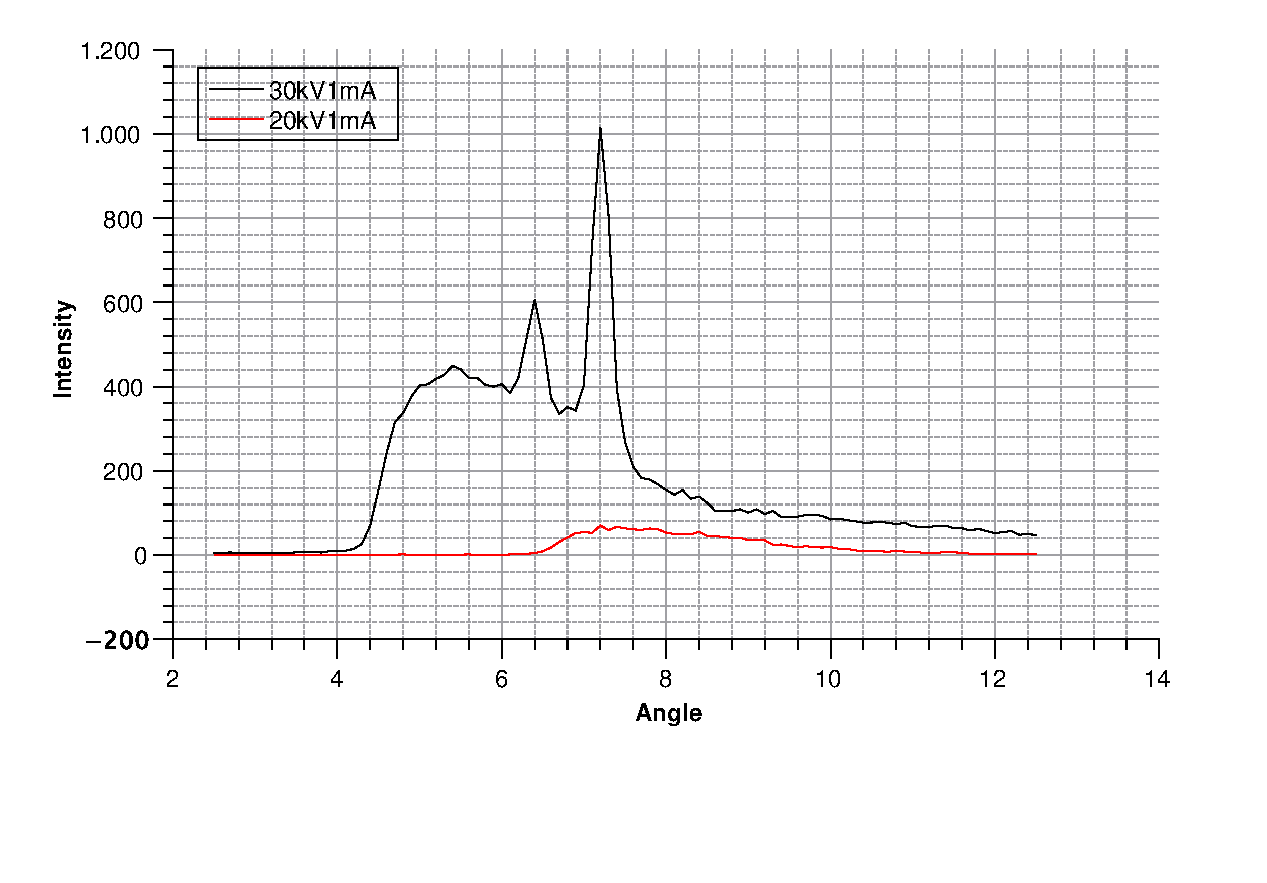
\includegraphics[width=10cm]{Influence_20_30.eps}
    \caption{Comparison of the intensity as a function of the angle, for two different tube high voltages}
    \label{fig:20_30}
\end{figure}
\FloatBarrier

\begin{figure}[!ht]
    \centering
    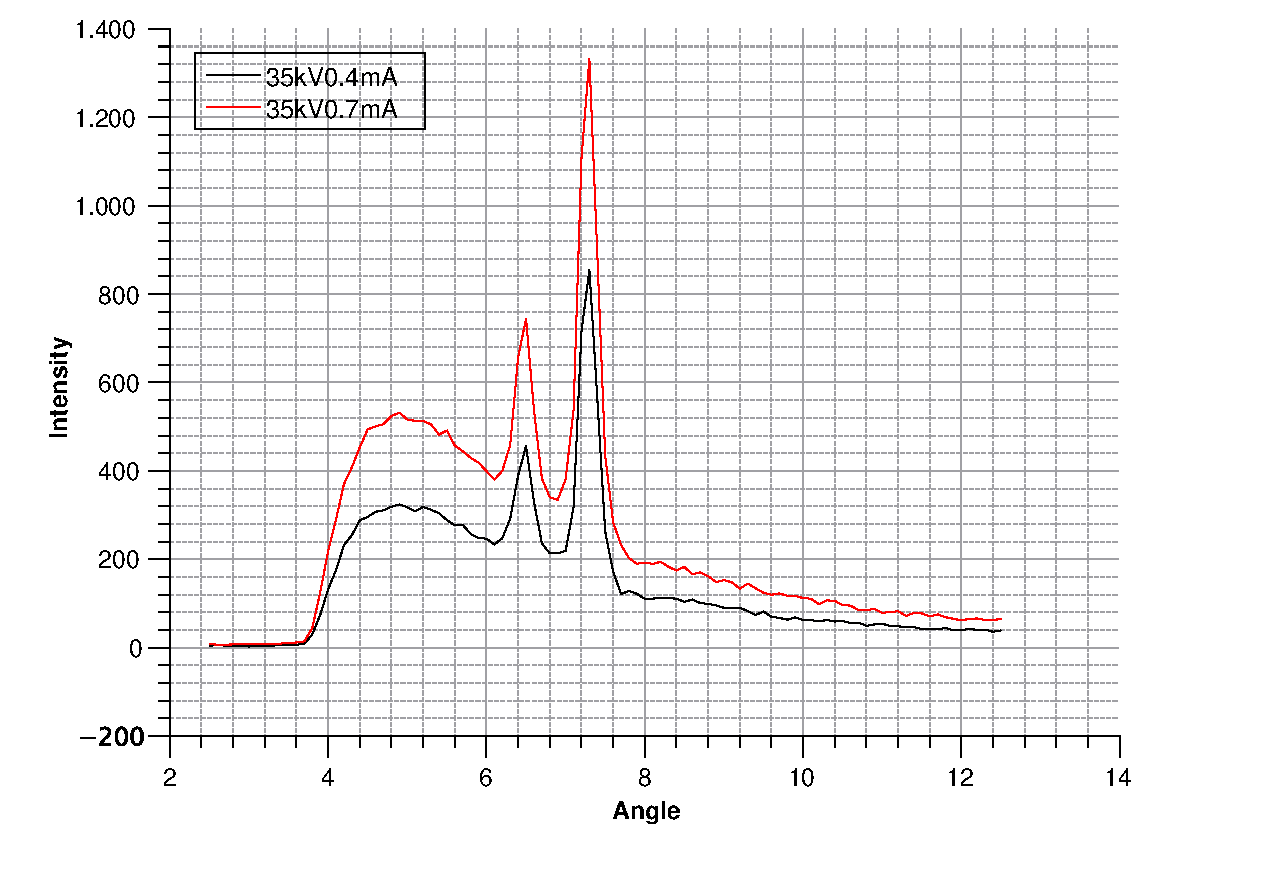
\includegraphics[width=10cm]{Inflience_35.eps}
    \caption{Comparison of the intensity as a function of the angle, for two different emission currents}
    \label{fig:35}
\end{figure}
\FloatBarrier

\noindent We notice that the higher the voltage, the higher the detected intensity. A certain voltage is needed to be able to see the a real spectrum with characteristic peaks which are not visible. At a tube high voltage of 20 kV on figure \ref{fig:20_30} we can't see the peaks. This is due to the electrons not having enough kinetic energy when they hit the anode to produce X-rays. Another observation is that the minimal wavelength is shifted to the right for lower voltages. \\ Additionally, the higher the emission current, the higher the detected intensity as one can see on figure \ref{fig:35}. As the material of the anode stays the same, the positions of the $K_{\alpha}$ and $K_{\beta}$ peaks stay the same. \\

\noindent Einstein called the X-ray production the inverse photoelectric effect. In the photoelectric effect, one shines light (or other electromagnetic radiation) onto a cathode, which then releases electrons and produces an electric current, if the electrons kinetic energy is high enough. When the frequency of the light is increased, the kinetic energy of the electrons is increased too. During X-ray production, it is the inverse phenomenon we are using: a current of electrons hits the anode, which, if the energy of the electrons is high enough, emits electromagnetic radiation, ie. X-rays. If we increase the current, we increase the intensity of the emitted X-rays.

\subsection{Duane Hunt law} \label{sectionDuaneHunt}

\noindent The Duane Hunt law (equation~(\ref{duaneHunt})) gives us a relationship between the limiting minimal wavelength $\lambda_{min}$ of the X-rays and the tube high voltage $V$.
\begin{equation}
    \lambda_{min} = \frac{hc}{eV}
    \label{duaneHunt}
\end{equation} where $e = 1.602 \cdot 10^{-19}$ C is the electron charge, $c = 299792458$ $\text{m} \cdot \text{s}^{-1}$ is the speed of light and $h$ is Planck's constant. The Duane-Hunt law can be rearranged into equation~(\ref{duaneHuntRewrite}). \begin{equation} h = \frac{\lambda_{min} \cdot eV}{c} \label{duaneHuntRewrite}\end{equation} which we can use to determine Planck's constant

\noindent We perform again several $\theta-2\theta$ scans with the parameters from table~(\ref{tab:parametersDuaneHunt}). They focus on the low $\theta$ part of the spectrum.

\begin{table}[!ht]
    \centering
    \begin{tabular}{c|c|c|c|c|c}
    Voltage (kV) & Current (mA) & $\Delta \beta$ & $\beta_{min}$   &  $\beta_{max}$   &  Acquisition time (s) \\ \hline
    25  & 1 & 0,1° & 3,2° & 6,2° & 30 \\
    30 & 1 & 0,1° & 3,2° & 6,2° & 30 \\
    35 & 1 & 0,1° & 3,2° & 6,2° & 30
    \end{tabular}
    \caption{Parameters applied on the X-ray tube for the determination of Planck's constant}
    \label{tab:parametersDuaneHunt}
\end{table}
\FloatBarrier

\noindent The resulting data can be seen in figure~(\ref{fig:duaneHunt}). Due to the experimental nature of the data, we have some noise remaining, and the curves don't quite reach an intensity of. Theoretically, the tail of the curve straightens; this behaviour is approximated by the linear fits for each curve, which is done on the steepest part.. The intersect with the 0 intensity line gives us the angle, and then by Bragg's law (equation~(\ref{braggLaw})) the minimal wavelength $\lambda_{min}$.

\begin{figure}[!ht]
    \centering
    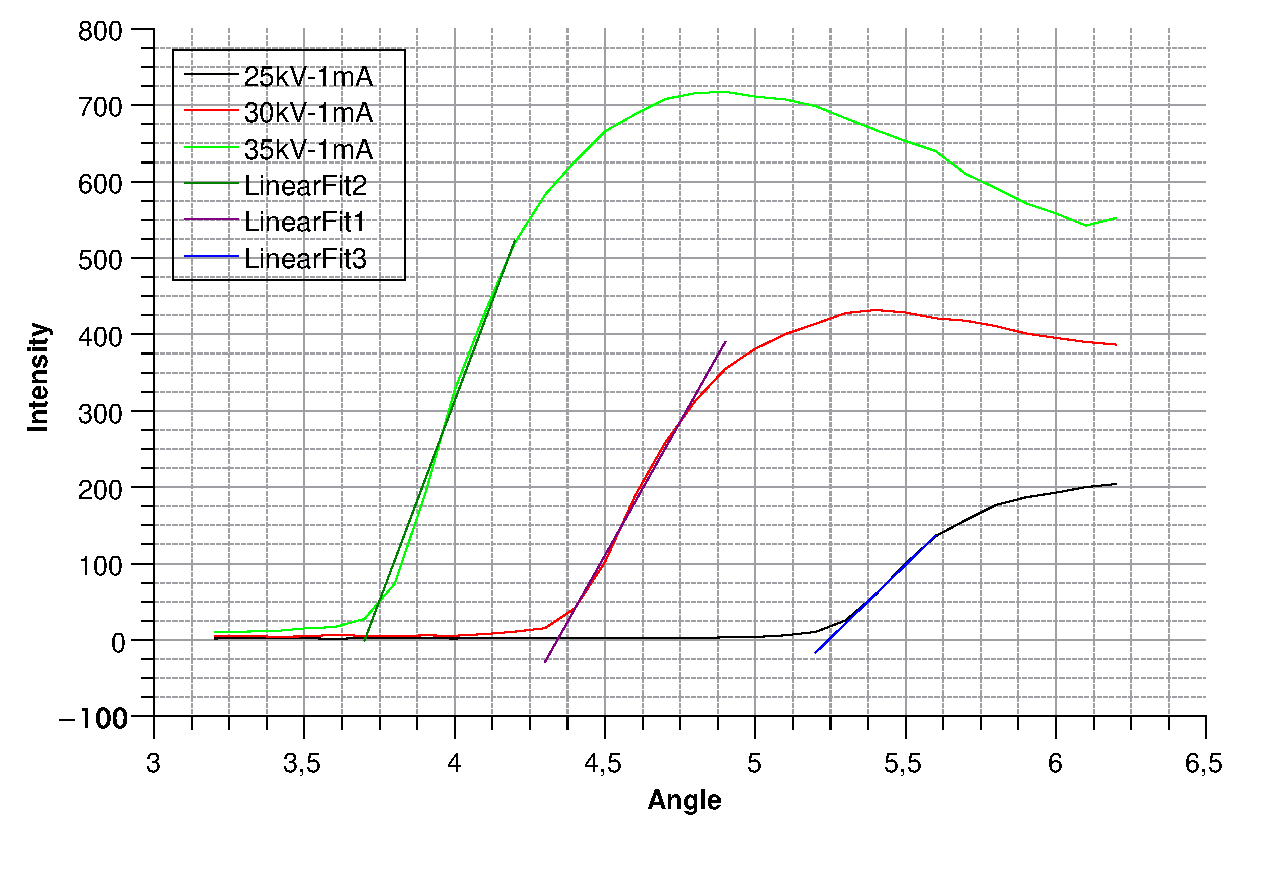
\includegraphics[width=10cm]{DuaneHunt_2.eps}
    \caption{Intensity as a function of angle for different high tube voltages}
    \label{fig:duaneHunt}
\end{figure}


\noindent The resulting minimal wavelength $\lambda_{min}$ for each curve can be found in table~(\ref{tab:duaneHuntMinWavelength}).

\begin{table}[!ht]
    \centering
    \begin{tabular}{c|c|c}
    Voltage (kV) & $\beta$  &  $\lambda_{min} (10^{-11} \ \text{m})$  \\ \hline
    25  & 5,3° & 5,03 \\
    30 & 4,3° &  4,08 \\
    35 & 3,7° &  3,51     
    \end{tabular}
    \caption{ Found angle and cutoff wavelength for their corresponding voltages}
    \label{tab:duaneHuntMinWavelength}
    \end{table}
\FloatBarrier

\noindent We can now insert these values into equation~(\ref{duaneHuntRewrite}), which gives an average of: \[\boxed{\overline{h_{exp}} = 5,61 \cdot 10^{-34}\ \text{Js}}\]

\noindent The relative error to the theoretical value $h_{th} = 6,62 \cdot 10^{-34} Js$ is:
\[\frac{\Delta h}{h_{exp}} = 18,1 \% \]

\subsection{Mosley's law}

\noindent For this part, we perform multiple $\theta-2\theta$ scans with different materials in front of the detector, so that X-rays will partially be absorbed. We have at our disposal Zr, Mo, Ag and In absorbers. With this data, we can determine Rydberg's constant using Mosley's law defined as:
\begin{equation}
    \lambda_K = \frac{1}{R(Z-1)^2}
\end{equation}
$\lambda_K$ being the critical wavelength, Z the atomic number and R Rydberg's constant. To obtain the critical wavelength, the same procedure as in section~(\ref{sectionDuaneHunt}) is used with the linear fit. We can rearrange this expression to give us \begin{equation}
    \frac{1}{\sqrt{\lambda_K}} = \sqrt{R}(Z-1)
    \label{mosleyLawRewrite}
\end{equation}

\noindent The parameters for the scans are presented in table~(\ref{tab:parametersMosley}).
\begin{table}[!ht]
    \centering
    \begin{tabular}{c|c|c|c|c|c}
    Voltage (kV) & Current (mA) & $\Delta\beta (^{\circ})$  & $\beta_{min} (^{\circ})$  &  $\beta_{max} (^{\circ})$   &  Acquisition time (s) \\ \hline
    35 & 1 & 0,1 & 3,5 & 7,8 & 5 
    \end{tabular}
    \caption{Parameters applied on the X-ray tube for the determination of Rydberg's constant}
    \label{tab:parametersMosley}
\end{table}

\noindent The resulting spectra with the different elements in front of the detector can be found in figure~(\ref{fig:spectraMosley})

\begin{figure}[!ht]
    \centering
    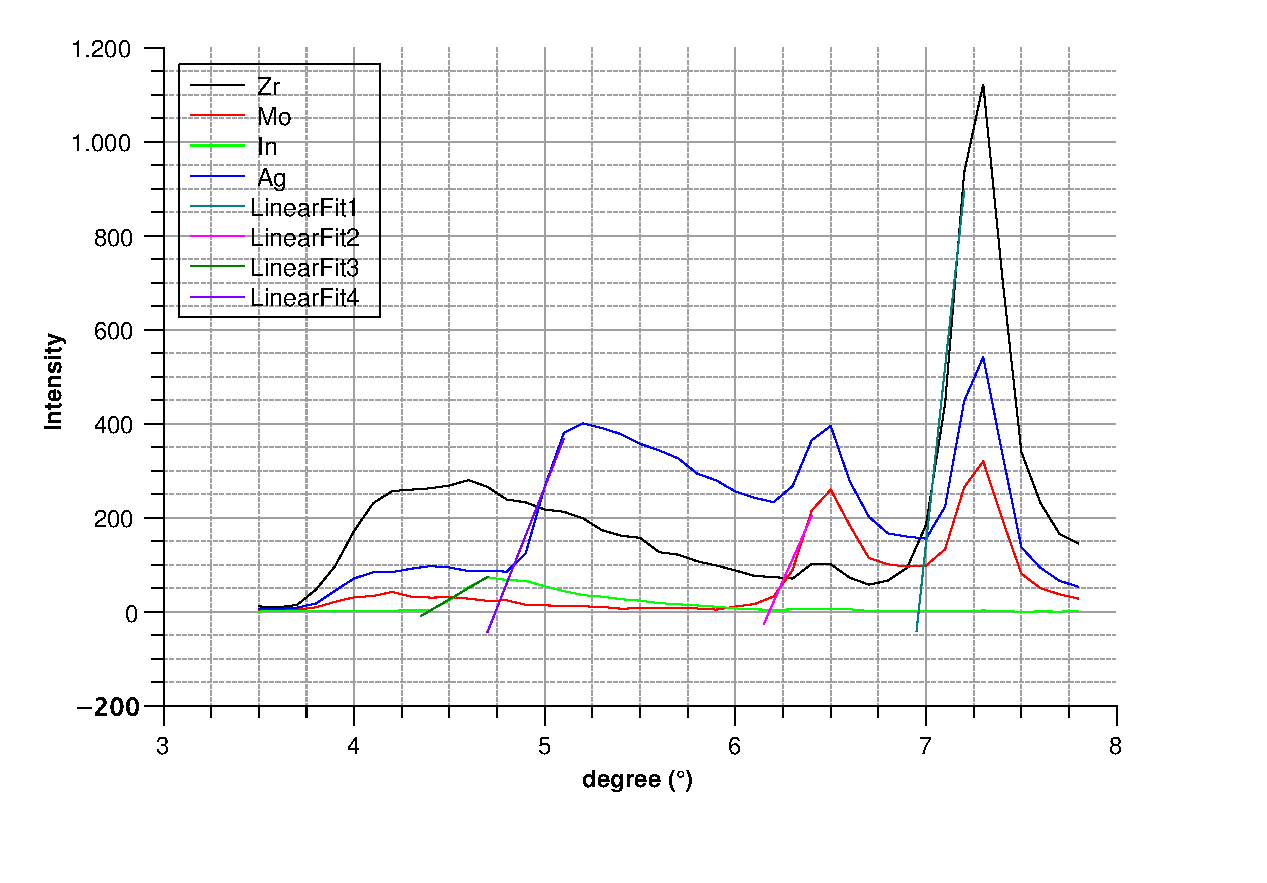
\includegraphics[width=12cm]{Mosley.eps}
    \caption{Bremsstrahlungsspectra with different absorbers in front of the detector, as a function of the angle}
    \label{fig:spectraMosley}
\end{figure}
\FloatBarrier

\noindent The corresponding critical wavelengths are presented in table~(\ref{tab:mosleyCritWavelength}).

\begin{table}[h]
    \centering
    \begin{tabular}{c|c|c|c}
    Element & Z & $\beta$  &  $\lambda (10^{-11} \ \text{m})$  \\ \hline
    Zr & 40 & 6,96° & 6,59   \\
    Mo & 42 & 6,18° & 5,86  \\
    Ag & 47 & 4,74° & 4,49  \\
    In & 49 & 4,40° & 4,17  
    \end{tabular}
    \caption{Absorber name with its atomic number, found minimal angle and calculated cutoff wavelength}
    \label{tab:mosleyCritWavelength}
\end{table}
\FloatBarrier

\noindent We can now use the equation~(\ref{mosleyLawRewrite}) to get a linear relationship between $\frac{1}{\sqrt{\lambda_K}}$ and $Z$. The results are plotted in figure~(\ref{fig:rydbergPlot}).

\begin{figure}[!ht]
    \centering
    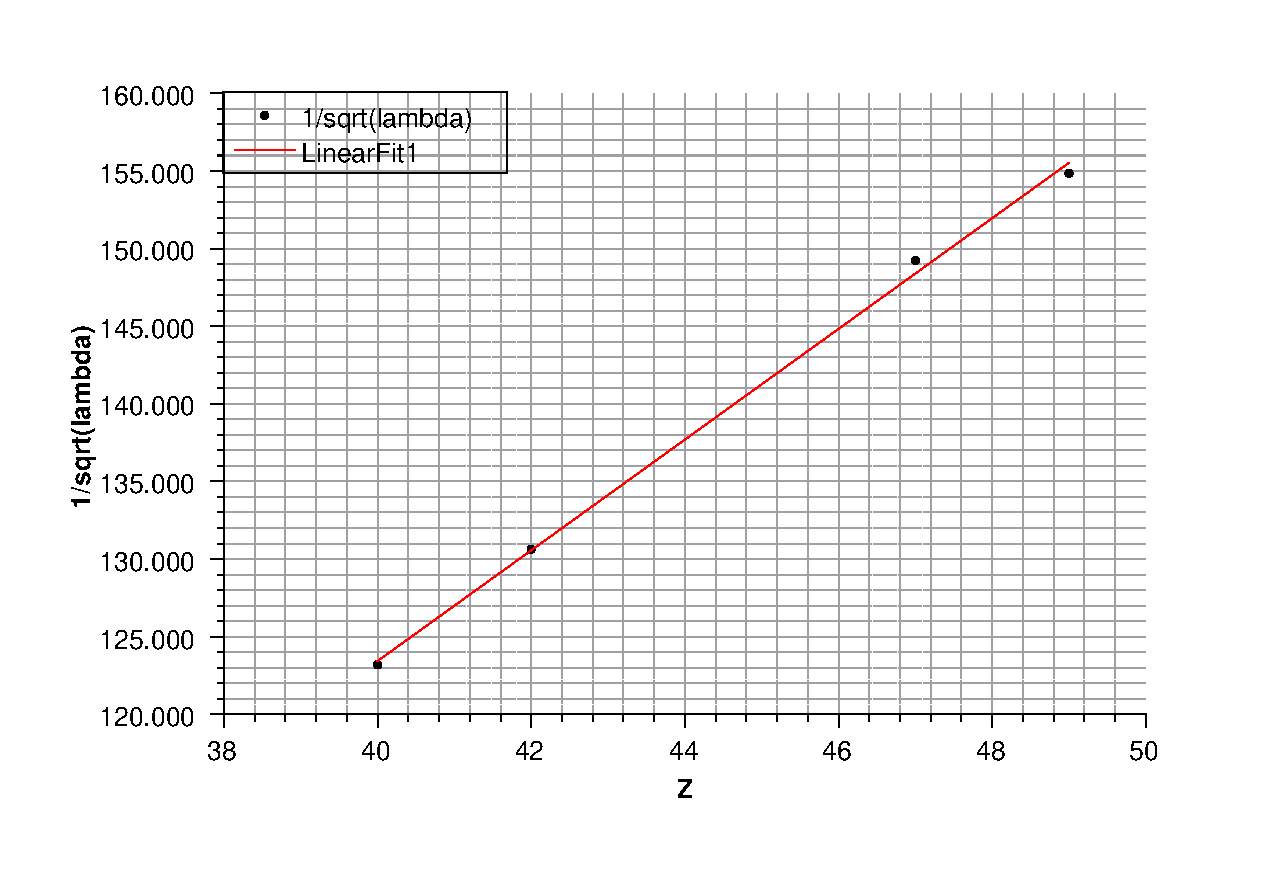
\includegraphics[width=10cm]{mosley_2.eps}
    \caption{Inverse square root of the wavelength as a function of Z}
    \label{fig:rydbergPlot}
\end{figure}
\FloatBarrier

\noindent The slope gives us the square root of the (experimental) Rydberg constant and squaring this value, we get:
\[\boxed{R_{exp} = 1,26 \cdot 10^7 \ \text{m}^{-1}}\]
Which has a deviation of 15,2$\%$ to the theoretical value $R_{th} = 1,097 \cdot 10^7 \ \text{m}^{-1}$

\subsection{Ionization by X-ray radiation}

\subsubsection{Ionization current $I_C$ as a function of the capacitor Voltage $V_C$}

\noindent The raw results of the experiment are shown in figure~(\ref{fig:IonizationCurrentAsFunctionOfCapacitorVoltage}).
\begin{figure}[!ht]
    \centering
    \resizebox{0.7\textwidth}{!}{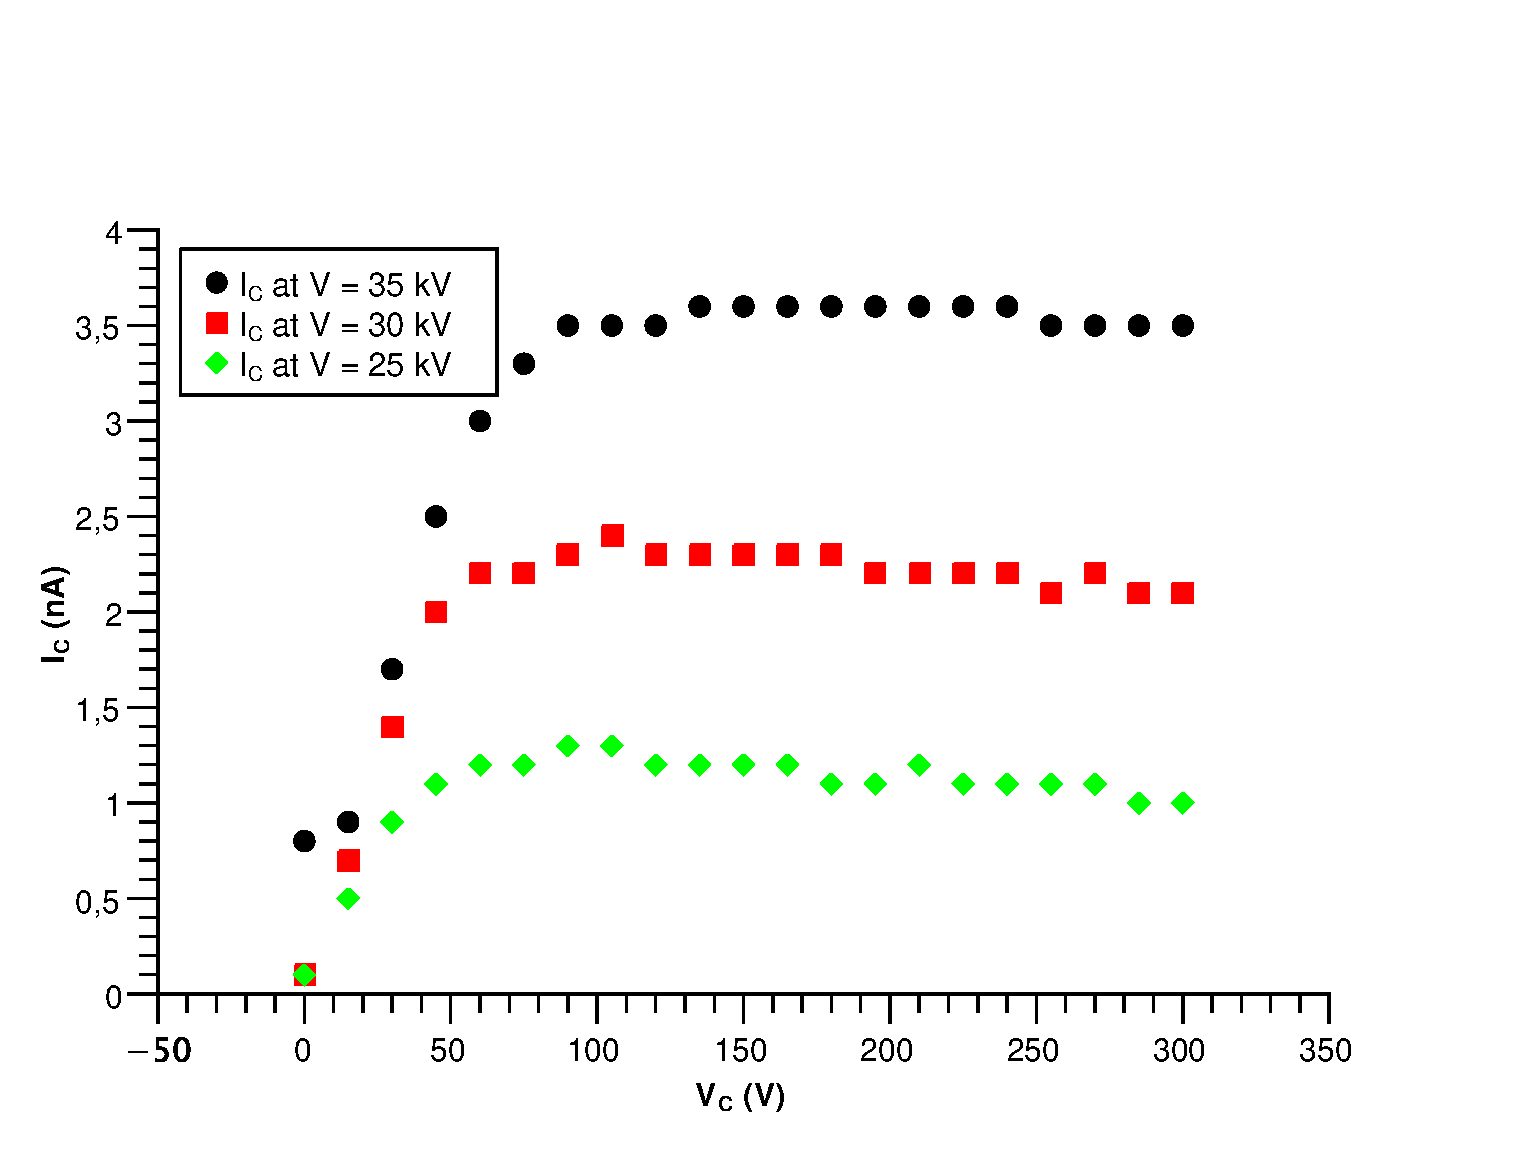
\includegraphics{IonizationCurrentAsFunctionOfCapacitorVoltage.eps}}
    \caption{Ionization current $I_C$ between the two plates as a function of the capacitor voltage $V_C$ at different tube voltages $V$}
    \label{fig:IonizationCurrentAsFunctionOfCapacitorVoltage}
\end{figure}
\FloatBarrier

\noindent We can now use the formula for the average ion dose rate $J$ of the air between the capacitor plates given by equation~(\ref{eq:ionDoseRate}):

\begin{equation}
    \left< J_{air} \right> = \frac{ \left< I_C \right>}{m_{air}}
    \label{eq:ionDoseRate}
\end{equation} 

\noindent The mass of the air between the plates can be calculated with $\rho_{air} \cdot V_{air}$, where $V_{air}$ is the volume between the two plates and $\rho_{air}$ is the density of the air. The volume between the plates is $V_{air} = 125 \ \text{cm}^3$~\cite{volumeCapacitor} and the density of the air is   $\rho_{air}=1.225 \ \text{kg} \cdot \text{m}^{-3}$ \cite{densityAir}. This gives $m_{air} = 1.531 \cdot 10^{-4} \ \text{kg}$. The resulting graph can be seen in figure~(\ref{fig:IonDoseRateAsFunctionOfCapacitorVoltage}).

\begin{figure}[!ht]
    \centering
    \resizebox{0.8\textwidth}{!}{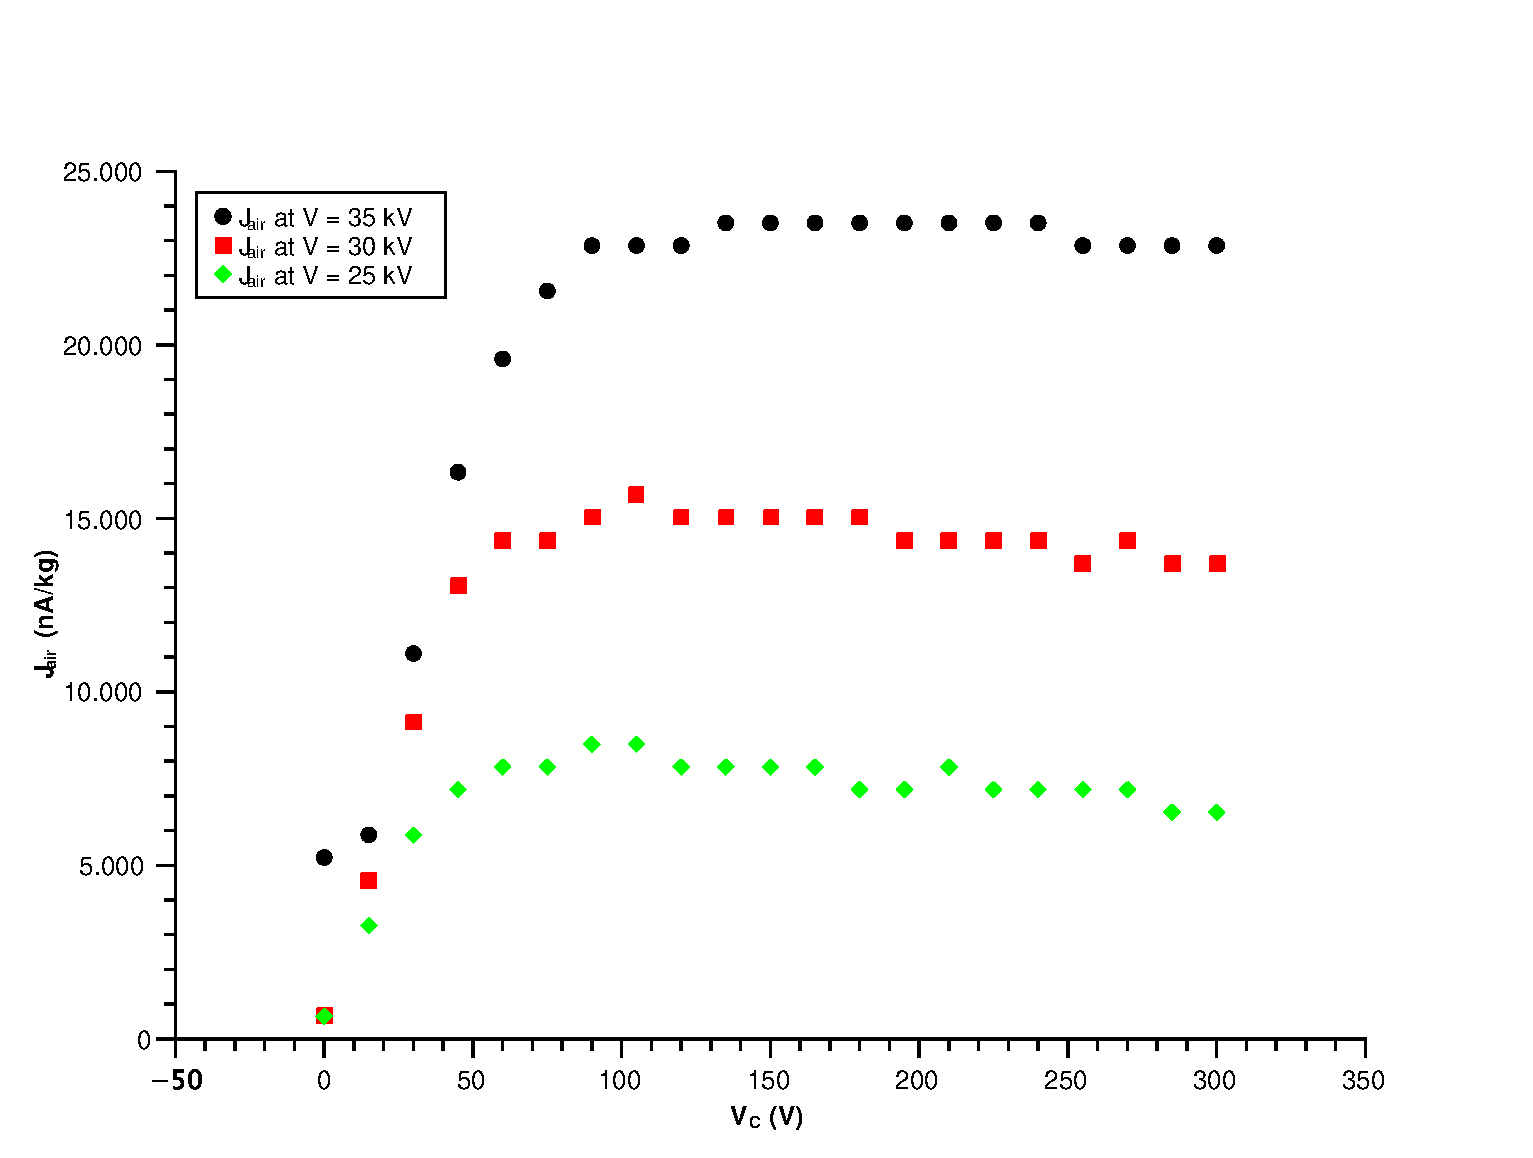
\includegraphics{IonDoseRateAsFunctionOfCapacitorVoltage.eps}}
    \caption{Ion dose rate of air $J_{air}$ as a function of the capacitor voltage $V_C$}
    \label{fig:IonDoseRateAsFunctionOfCapacitorVoltage}
\end{figure}
\FloatBarrier

\noindent We can observe, that the ion dose rate increases as the tube high voltage increases. This means the air gets more ionized and is a logical conclusion, since the higher the tube voltage is, the more energy the x-rays carry, and therefore the more ionization potential they have. It is also remarkable to see that after around 100 V, independently of the tube high voltage, the ion dose rate remains constant, and doesn't change much. This could maybe mean that the air is completely ionized.  

\subsubsection{Saturation ionization current $I_C$ as a function of the emission current I}

\noindent The results of the experiment can be found in figure~(\ref{fig:SaturationIonizationCurrentAsFunctionOfEmissionCurrent}). Note that the capacitor voltage is set to $V_C = 200$ V



\begin{figure}[!ht]
    \centering
    \resizebox{0.7\textwidth}{!}{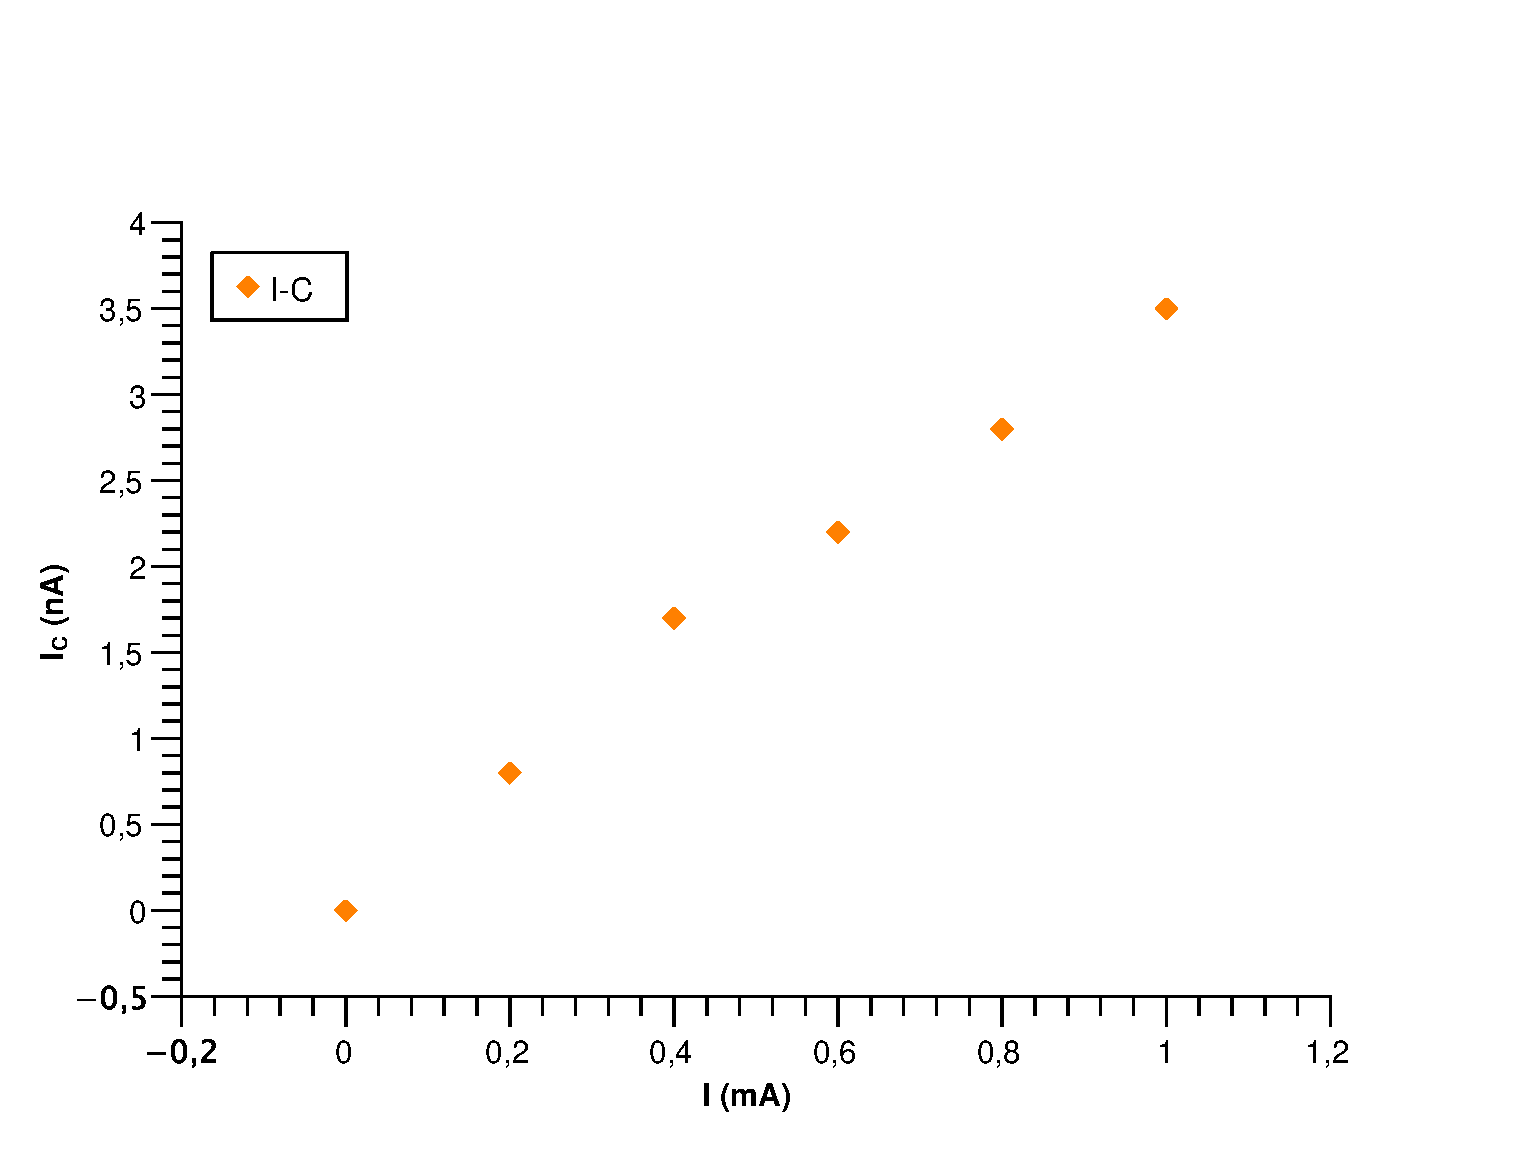
\includegraphics{SaturationIonizationCurrentAsFunctionOfEmissionCurrent.eps}}
    \caption{Saturation ionization current $I_C$ as a function of the emission current $I$}
    \label{fig:SaturationIonizationCurrentAsFunctionOfEmissionCurrent}
\end{figure}
\FloatBarrier


\noindent As previously, we can divide by the mass of the air inside the capcitor to obtain the saturation ion dose rate (see figure~(\ref{fig:SaturationIonDoseRateAsFunctionOfEmissionCurrent})). It scales linearly with the emission current. This means the more x-rays we produce, the higher the saturation ion dose gets.

\begin{figure}[!ht]
    \centering
    \resizebox{0.7\textwidth}{!}{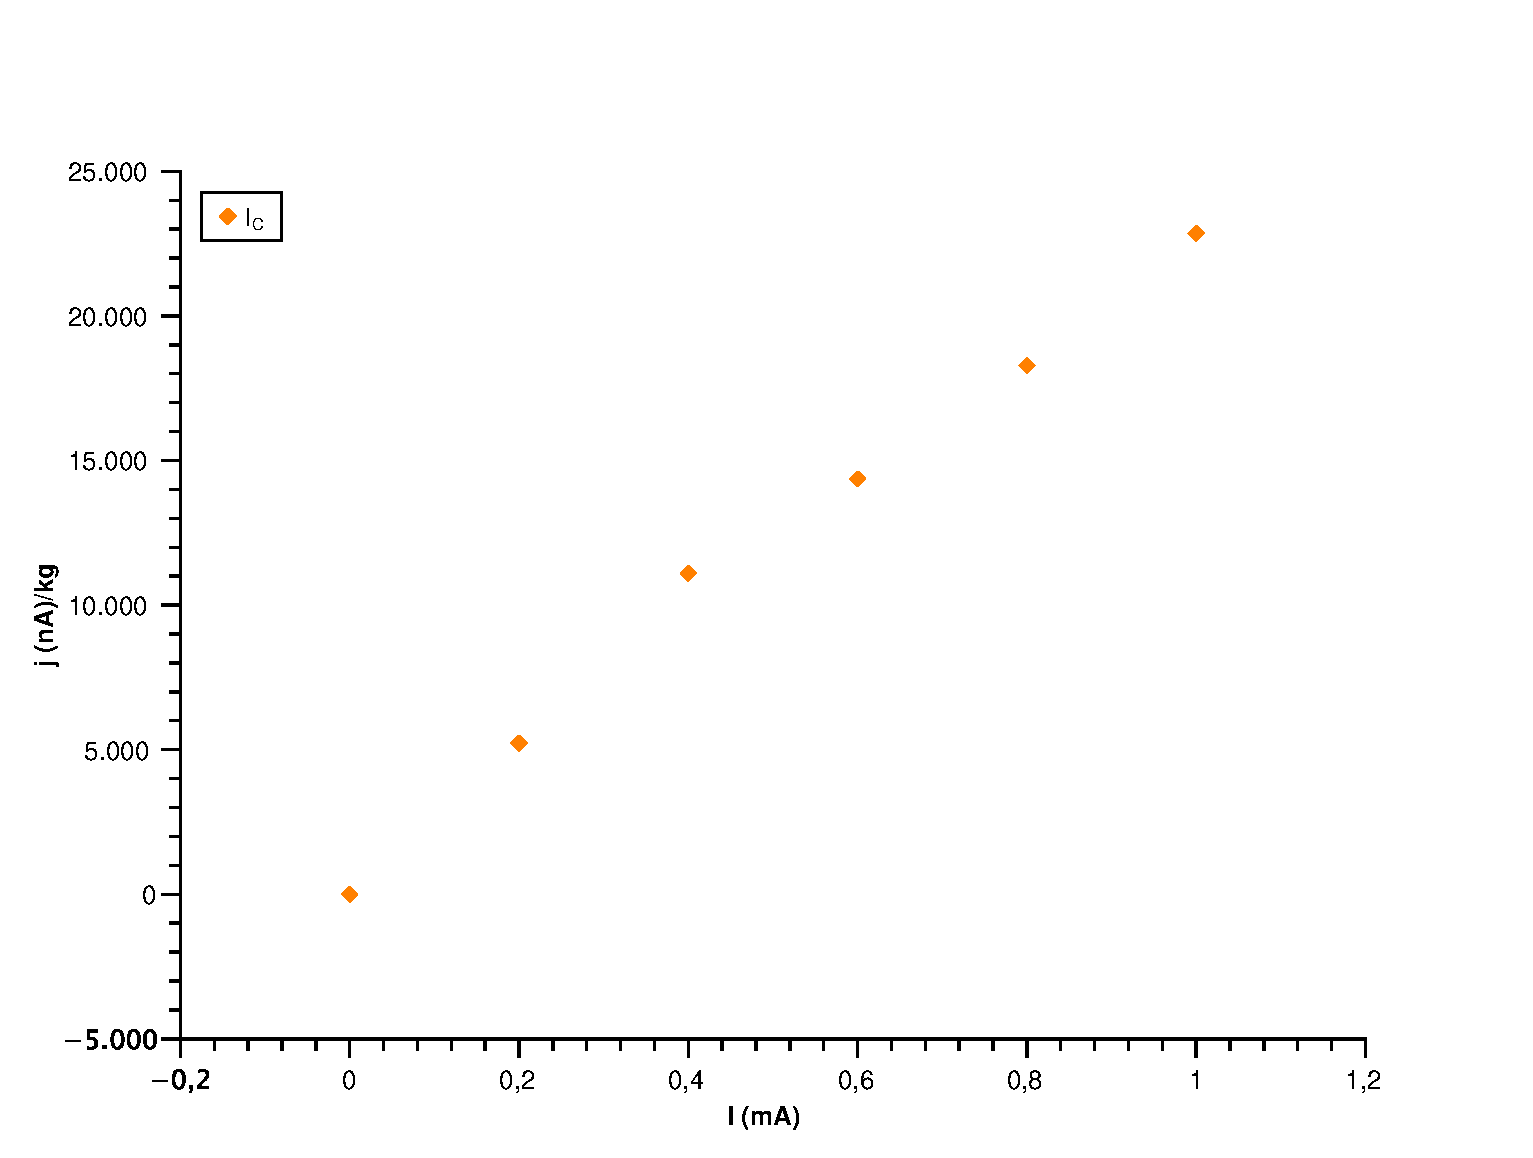
\includegraphics{SaturationIonizationCurrentAsFunctionOfEmissionCurrent2.eps}}
    \caption{Saturation ion dose rate $j$ as a function of the emission current $I$}
    \label{fig:SaturationIonDoseRateAsFunctionOfEmissionCurrent}
\end{figure}
\FloatBarrier

\subsubsection{Saturation ionization current $I_C$ as a function of the tube high voltage $V$}

\noindent The results of the experiment can be found in figure~(\ref{fig:SaturationIonizationCurrentAsFunctionOfTubeHighVoltage}). Note that the capacitor voltage is set to $V_C = 200$ V

\begin{figure}[!ht]
    \centering
    \resizebox{0.7\textwidth}{!}{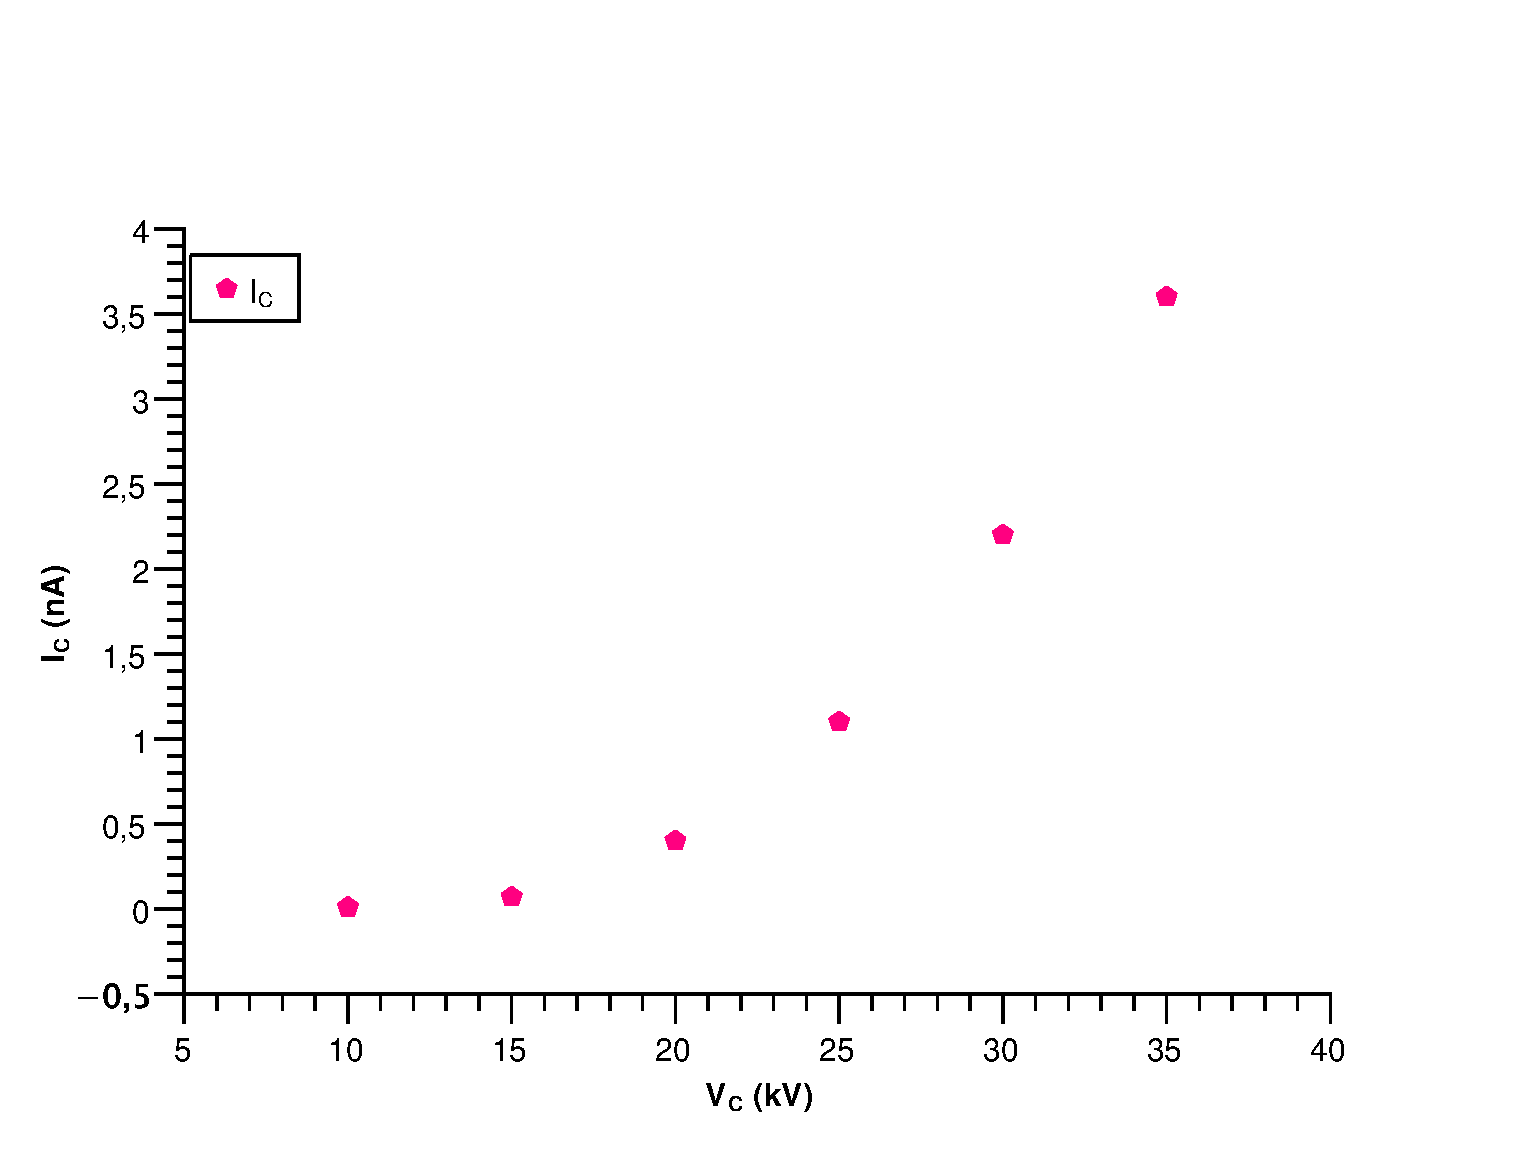
\includegraphics{SaturationIonizationCurrentAsFunctionOfTubeHighVoltage.eps}}
    \caption{Saturation ionization current $I_C$ as a function of the tube high voltage $V$}
    \label{fig:SaturationIonizationCurrentAsFunctionOfTubeHighVoltage}
\end{figure}
\FloatBarrier

\noindent Once again scaling by the factor $\frac{1}{m_{air}}$, we obtain the graph for the ion dose rate in figure~(\ref{fig:IonDoseRateAsFunctionOfTubeHighVoltage}) We can see that the the the ion dose rate grows faster for larger tube high voltages.

\begin{figure}[!ht]
    \centering
    \resizebox{0.7\textwidth}{!}{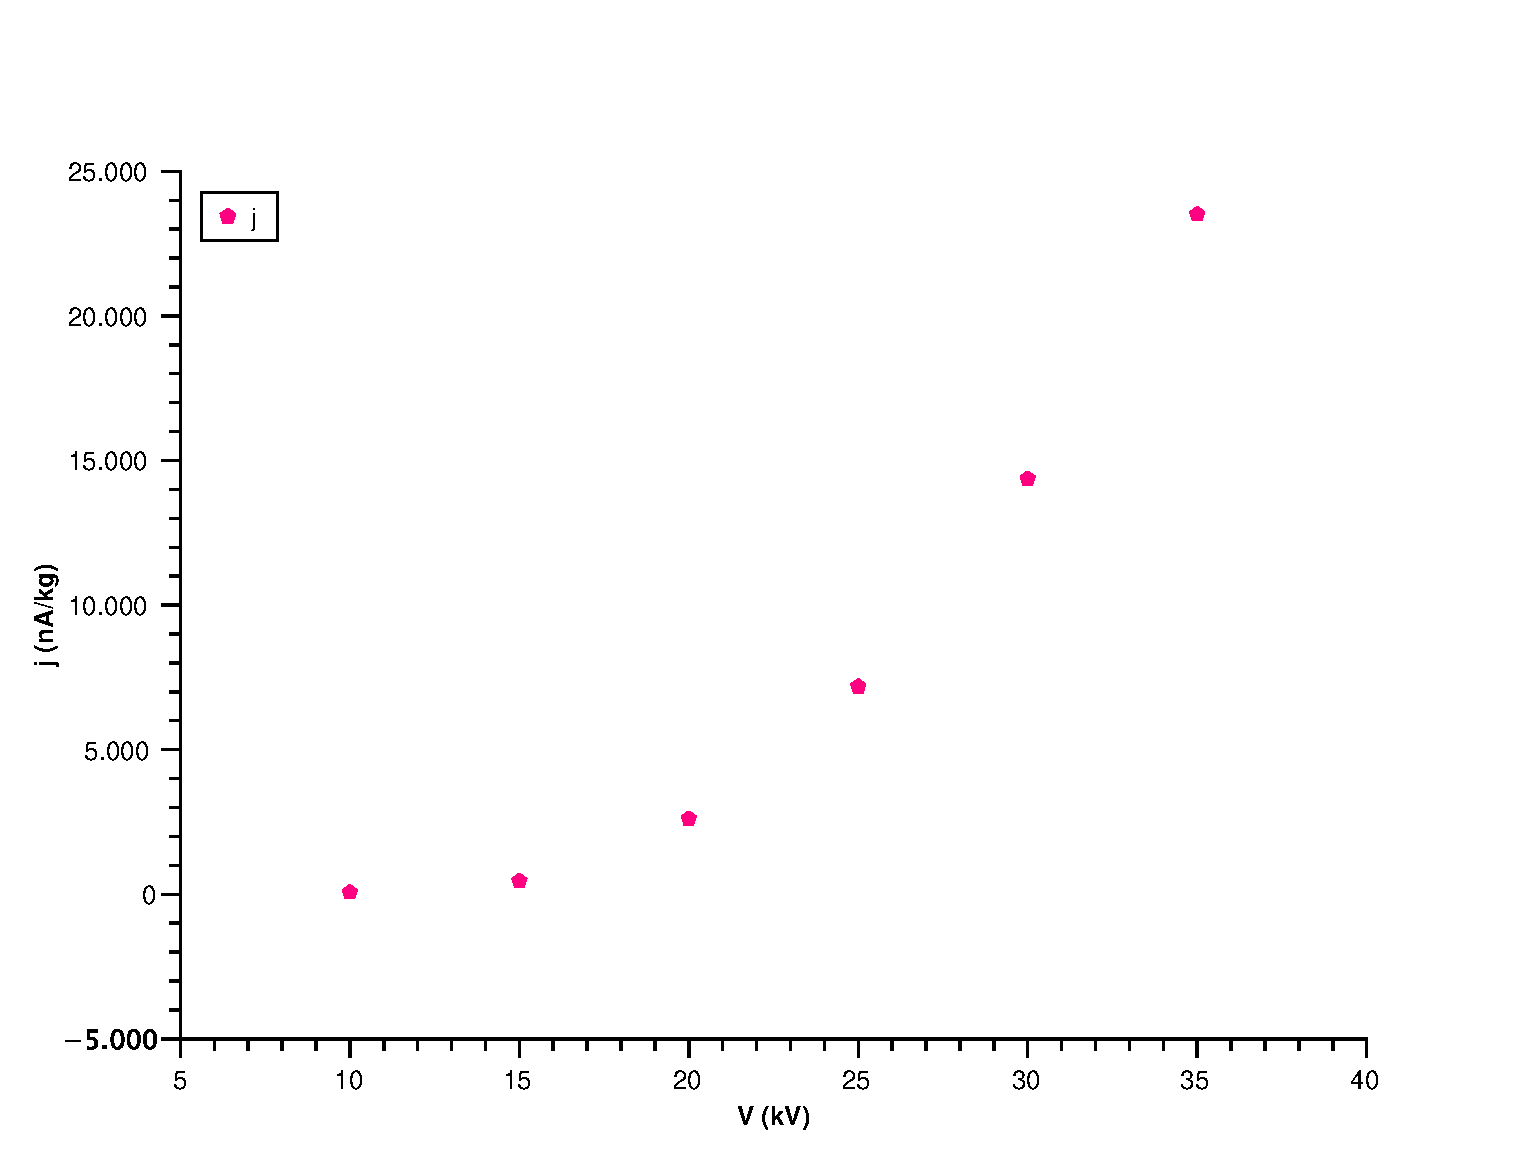
\includegraphics{SaturationIonizationCurrentAsFunctionOfTubeHighVoltage2.eps}}
    \caption{Ion dose rate $j$ as a function of the tube high voltage $V$}
    \label{fig:IonDoseRateAsFunctionOfTubeHighVoltage}
\end{figure}
\FloatBarrier

\clearpage

\subsection{Laue diagram}

\begin{wrapfigure}{r}{0.4\textwidth}
    \centering
    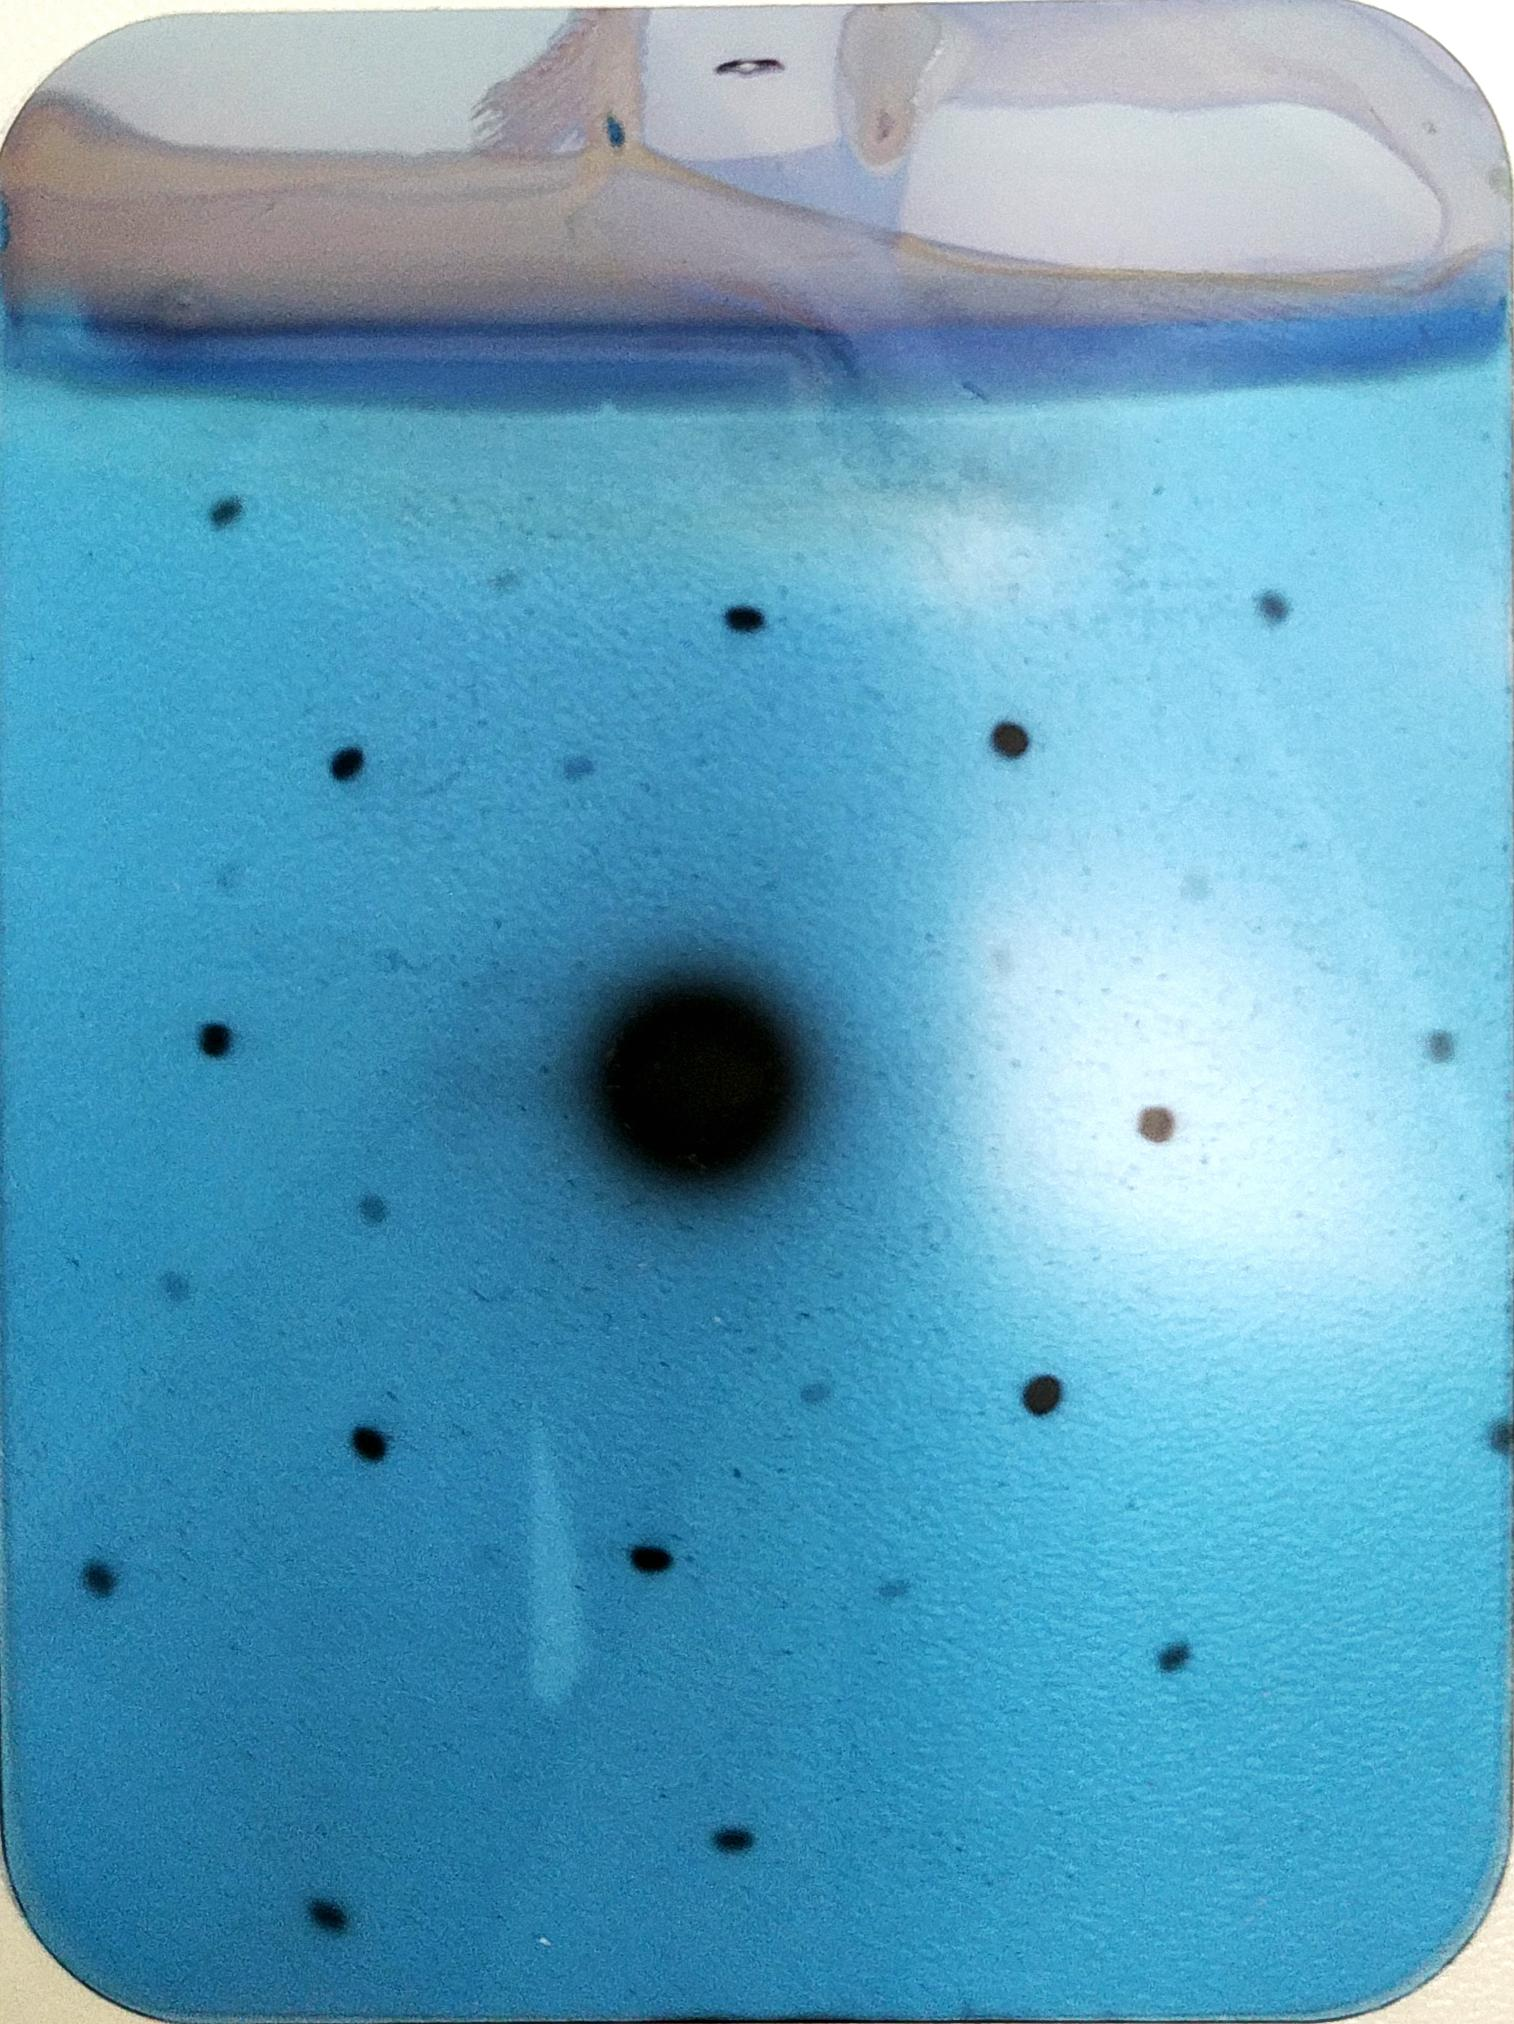
\includegraphics[width=5cm]{Laue Diagram.jpg}
    \caption{Laue diagram}
    \label{fig:laueDiagram}
\end{wrapfigure}
After letting the apparatus run for about 30 minutes, we develop the film, so that it doesn't react to light anymore and we can analyse the Laue diagram. In order to do so, it is put inside a darkroom, and successively dipped in a developer solution, rinsed in water, dipped in a fixer solution and finally rinsed with water again. The fully developed film can be seen in figure~(\ref{fig:laueDiagram}). The dots are created by "impacts" of the diffracted X-rays, and are related to the crystal structure and orientation. The brightness of the dots also varies. In our experiment, the diffracting crystal was a Lithium Fluoride crystal, and positioned in such a way, that its lattices are parallel to the photosensitive film. We will use this diagram to calculate the distance between two lattices of the LiF crystal, as well as the diffraction angle and the wavelengths of the diffracted X-rays. \\

\noindent Using the software "Geogebra", we can assign coordinates ($x_Q$,$y_Q$) to the points, in arbitrary units (see figure~(\ref{fig:laueCoordinates})). The real distance between the points J and F is exactly 3.5 cm, so we can rescale the coordinates to real values with the conversion factor $\frac{||J-F||_m}{||J-F||_{a.u.}}$. The $z_Q$ component can be found using \begin{equation}
    z_Q = \sqrt{x_Q^2+y_Q^2+L^2}-L
\end{equation} where $L$ is the distance between the crystal and the photosensitive film, in our case $L = 2.5$ cm. We  can then assign to each spot three integers $h, k, l,$, which are the three smallest integers, such that the proportion in equation (\ref{millerIndices}) holds: \begin{equation} h:k:l=x_Q:y_Q:z_Q \label{millerIndices} \end{equation} Next, the Bragg angle $\theta$ can be deduced by: \begin{equation}
    \theta = arctan \left( \frac{l}{\sqrt{h^2+k^2}} \right)
\end{equation} Finally, the wavelength $\lambda$ of the X-ray can be determined with the Bragg condition: \begin{equation}
    \lambda = 2dsin(\theta)
\end{equation} where $d$ is the distance between two lattices of the crystal and can be calculated with: \begin{equation}
    d = \frac{a_0}{\sqrt{h^2+k^2+l^2}}
\end{equation} where $a_0$ is the lattice constant of the crystal. For LiF crystals, the lattice constant is given by $a_0~=~402.8~\text{pm}$~\cite{latticeConstant}. The results are shown in table~(\ref{tab:laueRes}).

\begin{figure}[!ht]
    \centering
    \resizebox{\textwidth}{!}{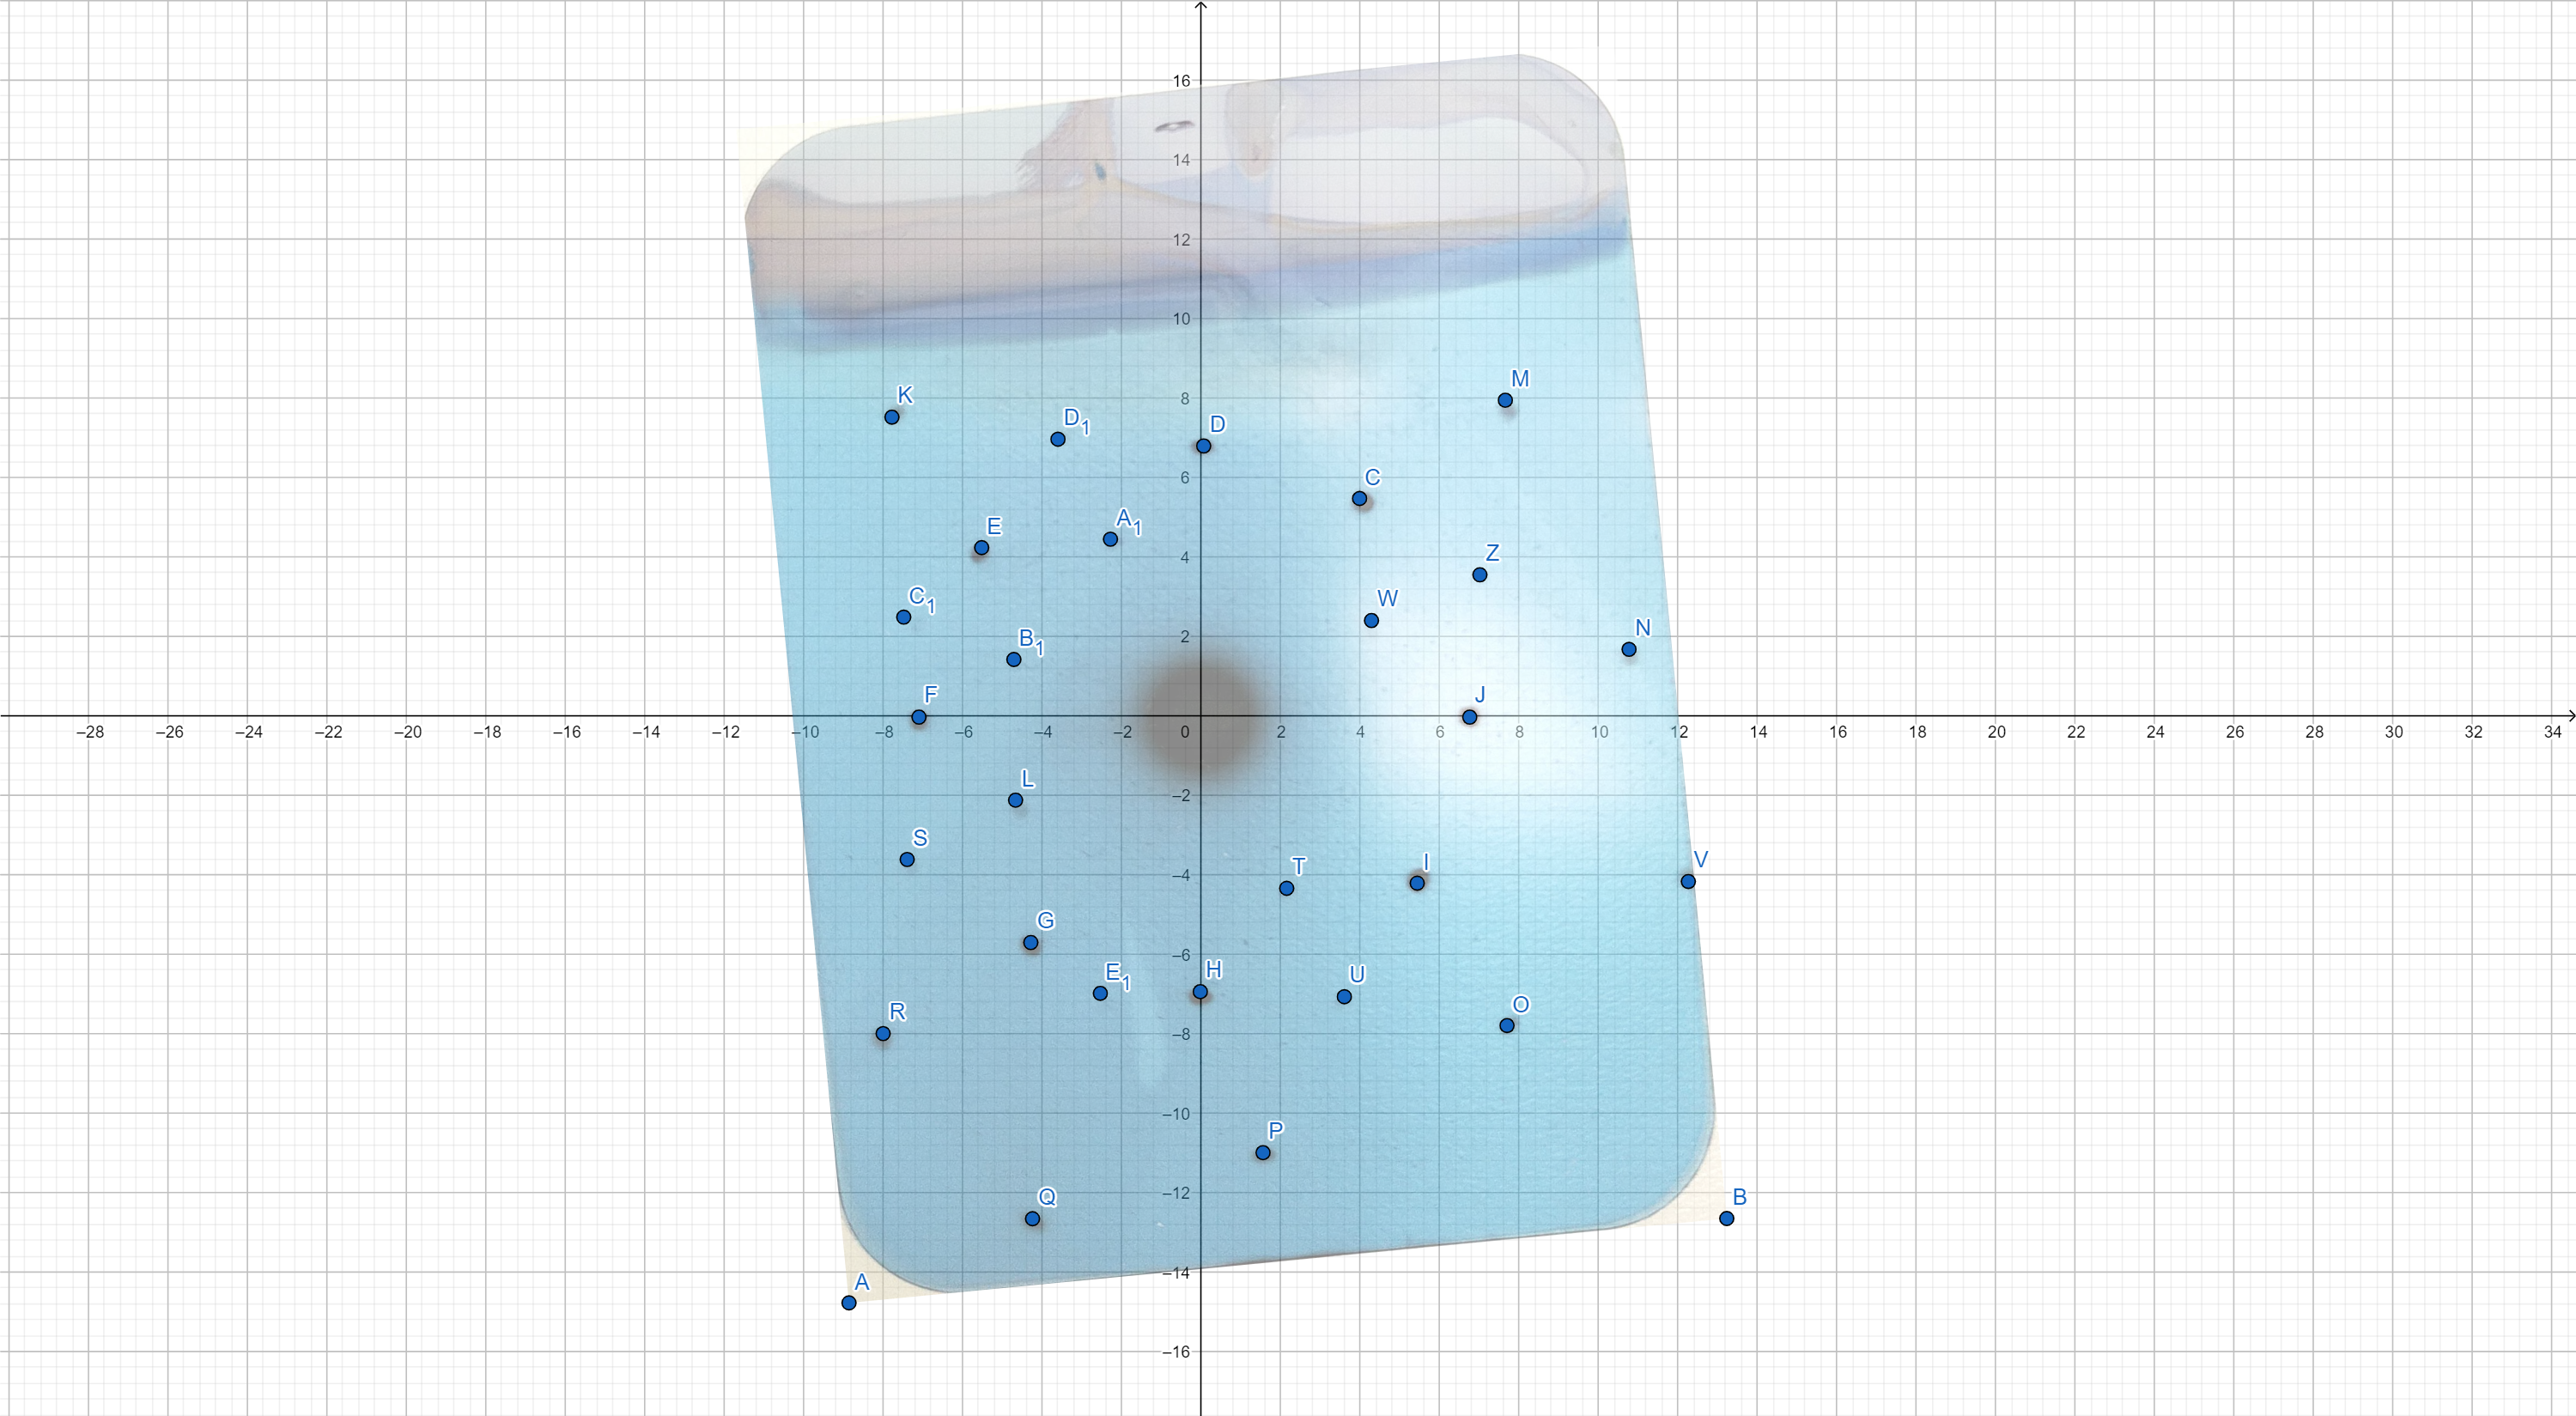
\includegraphics{geogebra-export.png}}
    \caption{Determination of the coordinates of the spots in GeoGebra (in arbitrary units)}
    \label{fig:laueCoordinates}
\end{figure}

\begin{table}[!ht]
    \centering
    \resizebox{\textwidth}{!}{\begin{tabular}{c|c|c|c|c|c|c|c|c|c|c|c}
        Point & x$_Q$ (a.u.) & y$_Q$ (a.u.)&  rescaled x$_Q$ (m) &  rescaled y$_Q$ (m) &  z$_Q$ (m)  & h & k & l & $\theta$ (°) & d (m) & $\lambda$ (m) \\ \hline
        A & -9 & -15 &  -0.0224 &  -0.0373 &  0.0252  & -2 & -3 & 4 & 0.837215003 & 7.47981 $\cdot 10^{-11}$ & 1.25244 $\cdot10^{-10}$  \\ 
        B & 13.23331 & -12.65433 &  0.0334  &  -0.0320 &  0.0276  & 3 & -3 & 4 & 0.75596941 & 6.90796 $\cdot10^{-11}$ & 1.04444 $\cdot10^{-10}$  \\ 
        C & 3.99117 & 5.46624 &  0.0101  &  0.0138  &  0.0053  & 3 & 4 & 5 & 0.785398163 & 5.69645 $\cdot10^{-11}$ & 8.94797 $\cdot10^{-11}$  \\ 
        D & 0.06728 & 6.78842 &  0.0002  &  0.0171  &  0.0053  & 0 & 1 & 1 & 0.785398163 & 2.84823 $\cdot10^{-10}$ & 4.47398 $\cdot10^{-10}$  \\ 
        E & -5.52 & 4.22936 &  -0.0139 &  0.0107  &  0.0056  & -4 & 3 & 5 & 0.785398163 & 5.69645  $\cdot 10^{-11}$ & 8.94797 $\cdot 10^{-11}$  \\ 
        F & -7.09809 & -0.03574 &  -0.0179 &  -0.0001 &  0.0058  & -1 & 0 & 1 & 0.785398163 & 2.84823 $\cdot 10^{-10}$ & 4.47398 $\cdot 10^{-10}$  \\ 
        G & -4.28312 & -5.70832 &  -0.0108 &  -0.0144 &  0.0058  & -3 & -4 & 5 & 0.785398163 & 5.69645 $\cdot 10^{-11}$ & 8.94797 $\cdot 10^{-11}$  \\ 
        H & -0.01802 & -6.9452 &  -0.0000 &  -0.0175 &  0.0055  & 0 & -1 & 1 & 0.785398163 & 2.84823 $\cdot 10^{-10}$ & 4.47398 $\cdot 10^{-10}$  \\ 
        I & 5.4413 & -4.21553 &  0.0137  &  -0.0106 &  0.0054  & 4 & 3 & 5 & 0.785398163 & 5.69645 $\cdot 10^{-11}$ & 8.94797 $\cdot 10^{-11}$  \\ 
        J & 6.76348 & -0.03574 &  0.0171  &  -0.0001 &  0.0053  & 1 & 0 & 1 & 0.785398163 & 2.84823 $\cdot 10^{-10}$ & 4.47398 $\cdot 10^{-10}$  \\ 
        K & -7.7805 & 7.51349 &  -0.0196 &  0.0190  &  0.0120  & -2 & 2 & 3 & 0.814826916 & 9.76933 $\cdot 10^{-11}$ & 1.59206 $\cdot 10^{-10}$  \\ 
        L & -4.66698 & -2.12563 &  -0.0118 &  -0.0054 &  0.0032  & -2 & -1 & 2 & 0.729727656 & 1.34267 $\cdot 10^{-10}$ & 1.95956 $\cdot 10^{-10}$  \\ 
        M & 7.65916 & 7.94 &  0.0193  &  0.0200  &  0.0124  & 2 & 2 & 3 & 0.814826916 & 9.76933 $\cdot 10^{-11}$ & 1.59206 $\cdot 10^{-10}$  \\ 
        N & 10.77268 & 1.6703 &  0.0272  &  0.0042  &  0.0122  & 7 & 1 & 7 & 0.780347572 & 4.04829 $\cdot 10^{-11}$ & 6.31815 $\cdot 10^{-11}$  \\ 
        O & 7.70181 & -7.79821 &  0.0194  &  -0.0197 &  0.0123  & 2 & -2 & 3 & 0.814826916 & 9.76933 $\cdot 10^{-11}$ & 1.59206 $\cdot 10^{-10}$  \\ 
        P & 1.56006 & -10.99704 &  0.0039  &  -0.0278 &  0.0126  & 1 & 7 & 7 & 0.780347572 & 4.04829 $\cdot 10^{-11}$ & 6.31815 $\cdot 10^{-11}$  \\ 
        Q & -4.24047 & -12.66043 &  -0.0107 &  -0.0320 &  0.0170  & -1 & 3 & 3 & 0.759070209 & 9.24087 $\cdot 10^{-11}$ & 1.40289 $\cdot 10^{-10}$  \\ 
        R & -8 & -8 &  -0.0202 &  -0.0202 &  0.0130  & 2 & 2 & 3 & 0.814826916 & 9.76933 $\cdot 10^{-11}$ & 1.59206 $\cdot 10^{-10}$  \\ 
        S & -7.39664 & -3.61842 &  -0.0187 &  -0.0091 &  0.0075  & -2 & 1 & 2 & 0.729727656 & 1.34267 $\cdot 10^{-10}$ & 1.95956 $\cdot 10^{-10}$  \\ 
        T & 2.15718 & -4.34349 &  0.0054  &  -0.0110 &  0.0028  & 1 & -2 & 2 & 0.729727656 & 1.34267 $\cdot 10^{-10}$ & 1.95956 $\cdot 10^{-10}$  \\ 
        U & 3.60731 & -7.07315 &  0.0091  &  -0.0179 &  0.0070  & 1 & 2 & 2 & 0.729727656 & 1.34267 $\cdot 10^{-10}$ & 1.95956 $\cdot 10^{-10}$  \\ 
        V & 12.26546 & -4.17288 &  0.0310  &  -0.0105 &  0.0162  & 3 & -1 & 3 & 0.759070209 & 9.24087 $\cdot 10^{-11}$ & 1.40289 $\cdot 10^{-10}$  \\ 
        W & 4.28973 & 2.39537 &  0.0108  &  0.0060  &  0.0029  & 2 & 1 & 2 & 0.729727656 & 1.34267 $\cdot 10^{-10}$ & 1.95956 $\cdot 10^{-10}$  \\ 
        Z & 7.01939 & 3.54695 &  0.0177  &  0.0090  &  0.0069  & 2 & 1 & 2 & 0.729727656 & 1.34267 $\cdot 10^{-10}$ & 1.95956 $\cdot 10^{-10}$  \\ 
        A1 & -2.27852 & 4.44262 &  -0.0058 &  0.0112  &  0.0030  & -1 & 2 & 2 & 0.729727656 & 1.34267 $\cdot 10^{-10}$ & 1.95956 $\cdot 10^{-10}$  \\ 
        B1 & -4.70963 & 1.4144 &  -0.0119 &  0.0036  &  0.0029  & -3 & 1 & 3 & 0.759070209 & 9.24087 $\cdot 10^{-11}$ & 1.40289 $\cdot 10^{-10}$  \\ 
        C1 & -7.48194 & 2.48067 &  -0.0189 &  0.0063  &  0.0070  & -3 & 1 & 3 & 0.759070209 & 9.24087 $\cdot 10^{-11}$ & 1.40289 $\cdot 10^{-10}$  \\ 
        D1 & -3.6007 & 6.95903 &  -0.0091 &  0.0176  &  0.0069  & -1 & 2 & 2 & 0.729727656 & 1.34267 $\cdot 10^{-10}$ & 1.95956 $\cdot 10^{-10}$  \\ 
        E1 & -2.53443 & -6.98785 &  -0.0064 &  -0.0176 &  0.0063  & -1 & -3 & 3 & 0.759070209 & 9.24087 $\cdot 10^{-11}$ & 1.40289 $\cdot 10^{-10}$ 
    \end{tabular}}
    \caption{Results of the analysis of the Laue diagram.  }
    \label{tab:laueRes}
\end{table}
\FloatBarrier

\noindent The majority of the wavelengths of the is in the $10^{-10}$ m range. Typically, X-rays have a wavelength of 0.1 \r{A} = $1 \cdot 10^-11$ m \cite{xrayWavelength}, but can actually range up to 10 nm \cite{xrayMaxWavelength}. Our calculated wavelengths fall into that range, and we can further certify that the produced electromagnetic waves by the Molybdenum anode are indeed X-rays.

\section{Conclusion}

This suite of experiment has allowed us to determine the Bremsstrahlungsspectrum of Molybdenum, study the characteristics of an X-ray tube, the Planck and Rydberg constants. We could also determine the ion dose rate of air due to ionization by X-rays. We determined the lattice structure of a Lithium Fluoride crystal and measured the wavelength of the emitted X-rays from the tube. \\ An area of improvement in this experiment is for the ionization of air. Since the currents are extremely small, it is difficult to make a precise measurement, the error is actually bigger than the value itself. Concerning the error, a personal improvement for this report would be to add error calculation where possible.

\section{Appendix}
\subsection{Theoretical values of the $K_{\alpha}$ and $K_{\beta}$ lines}
The energy for the transition from the level n to the level 1 is given by the formula:
\[ \Delta E = E_0(Z-1)^2\left(1-\frac{1}{n^2}\right) \]
Since for the $K_\alpha$ lines $n=2$ and for the $K_\beta$ lines $n=3$, this yields: \[\begin{cases}
    \Delta E_{K_\alpha} = E_0(Z-1)^2\left(1-\frac{1}{2^2}\right) \simeq 17,416.2 eV\\
    \Delta E_{K_\beta} = E_0(Z-1)^2\left(1-\frac{1}{3^2}\right) \simeq 20,321.4 eV 
\end{cases}\]
The corresponding wavelengths are given by \[ \lambda = \frac{hc}{\Delta E}\]
This yields:
\[\begin{cases}
    \lambda_{K_\alpha} = 7.231 \cdot 10^-2 \ nm \\
    \lambda_{K_\beta} = 6.101 \cdot 10^-2 \ nm
\end{cases}
\]
\subsection{Error calculation}
For additive (or substractive) formulae, of the form \[ X = A \pm B\] the error is : \[\Delta X = \Delta A + \Delta B\]
For multiplicative (or divisive) formulae of the form \[X = A \cdot  B^{\pm 1}\] the error ir: \[  \Delta X = X\sqrt{\left(\frac{\Delta A}{A}\right)^2+\left(\frac{\Delta B}{B}\right)^2} \]
For functional relationships: $Y=f(X)$ the error is: \[ \frac{\Delta Y}{Y} = \sqrt{\left|\frac{\partial f}{\partial X}\right|^2(\Delta X)^2} \] 

\begin{thebibliography}{!}
    \bibitem{volumeCapacitor} \textit{Detection of X-rays}, LD Didactics Gmbh, p.2 \url{https://www.ld-didactic.de/documents/en-US/EXP/P/P6/P6314_e.pdf?__hstc=98968833.be9877a1c87dd9d7496602e48835d89b.1648584423634.1648584423634.1648584423634.1&__hssc=98968833.1.1648584423634&__hsfp=3627262720&_ga=2.189090027.1728158462.1648584423-1121305948.1648584423}, accessed 30/03/22
    \bibitem{densityAir} \textit{Density of air}, Wikipedia, \url{https://en.wikipedia.org/wiki/Density_of_air}, accessed 30/03/22
    \bibitem{latticeConstant} Lab guide, p.16
    \bibitem{xrayWavelength} Lab guide, p.1
    \bibitem{xrayMaxWavelength} \textit{X-ray}, Wikipedia, \url{https://en.wikipedia.org/wiki/X-ray, consulted 30/03/22}
    \bibitem{braggLaw} Lab guide, p.7
\end{thebibliography}

\end{document}
